\documentclass{article}
\usepackage[utf8]{inputenc}
\usepackage[margin=1in]{geometry}
\usepackage{hyperref}
\usepackage{setspace}
\pagenumbering{arabic}
\usepackage{graphicx}
\usepackage[dvipsnames]{xcolor}
\usepackage{fancyhdr} 
\usepackage{amsmath, amsfonts, amsthm, amssymb}
\usepackage{bbm}
\usepackage{nth}
\usepackage{dsfont}
\usepackage{subfig}
\usepackage{tikz}
\usepackage{accents}


% commenting
\newcommand{\comment}[3]{\textcolor{#1}{\textbf{[#2: }\textit{#3}\textbf{]}}}
\newcommand{\emma}[1]{\comment{purple}{EK}{#1}}
\newcommand{\jesse}[1]{\comment{BurntOrange}{JG}{#1}}
\newcommand{\miaoshiqi}[1]{\comment{ForestGreen}{ML}{#1}}
\newcommand{\siyue}[1]{\comment{blue}{SY}{#1}}

%For references using Lemma, Theorem, etc, use \cref
\usepackage[nameinlink,capitalize,sort]{cleveref}

% theorems
\newtheorem{theorem}{Theorem}[section]
\newtheorem{lemma}[theorem]{Lemma}
\newtheorem{definition}[theorem]{Definition}
\newtheorem{proposition}[theorem]{Proposition}
\newtheorem{example}[theorem]{Example}
\newtheorem{corollary}[theorem]{Corollary}
%theoremstyle{plain} %boldface title, italicized body. Commonly used in theorems, lemmas, corollaries, propositions and conjectures.
%\theoremstyle{definition} %boldface title, Roman body. Commonly used in definitions, conditions, problems and examples
\theoremstyle{remark} %italicized title, Roman body. Commonly used in remarks, notes, annotations, claims, cases, acknowledgments and conclusions.
\newtheorem{exercise}[theorem]{Exercise}

\newenvironment{solution}
  {\renewcommand\qedsymbol{$\blacksquare$}\begin{proof}[Solution]}
  {\end{proof}}

% weird hack to get rid of dot:
\usepackage{xpatch}
\makeatletter
\AtBeginDocument{\xpatchcmd{\@thm}{\thm@headpunct{.}}{\thm@headpunct{}}{}{}}



% lin alg
\newcommand{\bu}{{\mathbf{u}}}
\newcommand{\bv}{{\mathbf{v}}}
\newcommand{\bw}{{\mathbf{w}}}
\newcommand{\bx}{\mathbf{x}}
\newcommand{\zerovec}{{\mathbf{0}}}

% other useful stuff
\newcommand{\Id}{{\mathds{1}}}
\newcommand{\N}{{\mathbb{N}}}
\newcommand{\R}{{\mathbb{R}}}
\newcommand{\C}{{\mathbb{C}}}
\newcommand{\Z}{{\mathbb{Z}}}
\newcommand{\Q}{{\mathbb{Q}}}
\newcommand{\F}{{\mathbb{F}}}
\newcommand{\cL}{{\mathcal{L}}}
\newcommand{\cP}{\mathcal{P}}
\newcommand{\inv}{{-1}}

%\DeclareMathOperator{\dim}{dim}
\DeclareMathOperator{\range}{range}
\DeclareMathOperator{\rank}{rank}
\DeclareMathOperator{\nullity}{nullity}

\hypersetup{
  colorlinks   = true, %Colours links instead of boxes
  urlcolor     = blue, %Colour for external hyperlinks
  linkcolor    = black, %Colour of internal links
  citecolor   = black %Colour of citations
}

\allowdisplaybreaks % fixes align environment weird spacing on page
\setlength{\parindent}{0cm}

% get rid of dot after theorem 
\usepackage{xpatch}
\makeatletter
% Patch to accommodate for \begin{theorem}[...]
\AtBeginDocument{\xpatchcmd{\cref@thmoptarg}{\thm@headpunct{.}}{\thm@headpunct{}}{}{}}
% Patch to accommodate \begin{theorem} (without an optional argument)
\AtBeginDocument{\xpatchcmd{\cref@thmnoarg}{\thm@headpunct{.}}{\thm@headpunct{}}{}{}}


% \usepackage[natbib=true, style=vancouver]{biblatex}
 \usepackage[backend= biber, style=vancouver]{biblatex}
\bibliography{references.bib}

\title{Mathematics Bootcamp Lecture Notes \\
\vspace{0.5em}
\large Department of Statistical Sciences, University of Toronto}
\author{Emma Kroell}
\date{Last updated: \today}

\begin{document}

\maketitle


\newpage
\section*{Preface}

These lecture notes were prepared for the Mathematics course at the inaugural Department of Statistical Sciences Graduate Student Bootcamp at the University of Toronto. The course taught an overview of necessary mathematics prerequisites to incoming statistics graduate students, with an emphasis on proofs.

\vspace{1em}

These lectures are based on the following books or lecture notes:

\vspace{1em}

1. \href{https://link-springer-com.myaccess.library.utoronto.ca/book/10.1007/978-1-4614-4265-3}{{\emph{An Introduction to Mathematical Structures and Proofs}}} by Larry J. Gerstein


2. \href{https://link-springer-com.myaccess.library.utoronto.ca/book/10.1007/0-387-28387-0}{\emph{A Taste of Topology}} by Volker Runde


3. \href{https://link-springer-com.myaccess.library.utoronto.ca/book/10.1007/978-3-319-11080-6}{{\emph{Linear Algebra Done Right}}} by Sheldon Axler

4. \href{https://www.math.brown.edu/streil/papers/LADW/LADW.html}{{\emph{Linear Algebra Done Wrong}}} by Sergei Treil


5. \href{https://digitalcommons.trinity.edu/mono/7/}{{\emph{Introduction to Real Analysis}}} by William F. Trench

6. \href{https://link-springer-com.myaccess.library.utoronto.ca/book/10.1007/978-1-4939-2712-8}{{\emph{Understanding Analysis}}} by Stephen Abbott

7. \href{https://link-springer-com.myaccess.library.utoronto.ca/book/10.1007/978-3-319-17771-7}{\emph{Real Mathematical Analysis}} by Charles C. Pugh

8. \href{http://84.89.132.1/~piotr/docs/RealAnalysisNotes.pdf}{\emph{Lecture notes in Mathematics for Economics and Statistics}} by Piotr Zwiernik

9. \href{http://www.math.uwaterloo.ca/~lwmarcou/notes/pmath351.pdf}{{\emph{Real Analysis Lecture Notes}}} by Laurent Marcoux

\vspace{1em}

Chapter 1 of Gerstein (2012) is used a reference for the proof technique section. Runde (2005) is the main text for the sections on set theory, metric spaces, and topology, which follow chapters 1, 2, and 3 of his book, respectively. The linear algebra content comes mostly from Axler (2015), with Treil (2017) used in some sections for an alternate perspective.

\vspace{1em}

The material in these notes belongs to these texts. All of these texts are available online to University of Toronto users (some to everyone).

\vspace{1em}

I would like to acknowledge Jesse Gronsbell, Stanislav Volgushev, Piotr Zwiernik, and Robert Zimmerman for their assistance in developing the list of topics for the course. 

\newpage
\tableofcontents


\newpage
\section{Review of proof techniques}
\subsection{Propositional logic}

{\bf Propositions} are statements that could be true or false. They have a corresponding {\bf truth value}.We will use capital letters to denote propositions. 

\vspace{1em}

ex. ``$n$ is odd'' and ``$n$ is divisible by 2'' are propositions . 

Let's call them $P$ and $Q$. Whether they are true or not (i.e. their truth value) depends on what $n$ is. 

\vspace{1em}

We can  negate statements: $\neg P$ is the statement ``$n$ is not odd''

\vspace{1em}
 We can combine statements: 
 \begin{itemize}
 \item $P \wedge Q$ is the statement ``$n$ is odd and $n$ is divisible by 2''.
 \item $P \vee Q$ is the statement ``$n$ is odd or $n$ is divisible by 2''. We always assume the inclusive or unless specifically stated otherwise.
\end{itemize}

Examples:
\begin{itemize}
              \item If it's not raining, I won't bring my umbrella.
              \item I'm a banana or Toronto is in Canada.
              \item If I pass this exam, I'll be both happy and surprised.
\end{itemize}


\subsubsection{Truth values}

\begin{example} Write the following using propositional logic
If it is snowing, then it is cold out. \\
It is snowing. \\
Therefore, it is cold out.  
\end{example}

\begin{solution}
$P \implies Q$ \\
$P$ \\
Conclusion: $Q$ \\
\end{solution}


To examine if statement is true or not, we use a truth table


\begin{tabular}{|c|c| c|}
\hline
     $P$& $Q$ &  $P \implies Q$ \\ \hline
     T& T & T \\ \hline
     T & F & F \\ \hline
     F & T & T \\ \hline
     F & F & T \\ \hline
\end{tabular}



\subsubsection{Logical equivalence}

\begin{tabular}{|c|c| c|}
\hline
     $P$& $Q$ &  $P \implies Q$ \\ \hline
     T& T & T \\ \hline
     T & F & F \\ \hline
     F & T & T \\ \hline
     F & F & T \\ \hline
\end{tabular} \hspace{2cm} \begin{tabular}{|c | c | c | c|}
\hline
     $P$& $Q$ & $\neg P$ & $\neg P \vee Q$  \\ \hline
     T& T & F & T \\ \hline
     T & F & F & F \\ \hline
     F & T &  T &T \\ \hline
     F & F & T & T \\ \hline
\end{tabular}


What is $\neg (P \implies Q)$?



\subsection{Types of proof}
\begin{itemize}
	\item Direct
	\item Contradiction
	\item Contrapositive
	\item Induction
\end{itemize}


\subsubsection{Direct Proof}

{\bf Approach:} Use the definition and known results.
\vspace{1em}

\begin{example}
The product of an even number with another integer is even.
\end{example}

Approach: use the definition of even.

\begin{definition}
We say that an integer $n$ is {\bf even} if there exists another integer $j$ such that $n=2j$. \\
We say that an integer $n$ is {\bf odd} if there exists another integer $j$ such that $n=2j+1$.
\end{definition}

\begin{proof}
Let $n, m \in \Z$, with $n$ even. By definition, there $\exists$ $j \in \Z$ such that $n = 2j$. Then 
$$ n m  =  (2 j) m = 2 (j m)$$
Therefore $n m$ is even by definition. 
\end{proof}

\begin{definition}
Let $a,b \in \Z$. We say that ``a divides b'', written $a | b$, if the remainder is zero when $b$ is divided by $a$, i.e. $\exists j \in \Z$ such that $b = a j$.
\end{definition}

% https://hsm.stackexchange.com/questions/5656/who-invented-the-divisibility-symbol-and-why-is-it-backwards

\begin{example}
Let $a,b,c \in \Z$ with $a \neq 0$. Prove that if $a | b$ and $b | c$, then $a | c$.
\end{example}
\begin{proof}
Suppose $a | b$ and $b | c$. Then by definition, there exists $j,k \in \Z$ such that $b = aj$ and $c = kb$. Combining these two equations gives $c = k (aj) = a (kj)$. Thus $a | c$ by definition.
\end{proof}

\subsubsection{Proof by contrapositive}
\begin{example}
If an integer squared is even, then the integer is itself even.
\end{example}


How would you approach this proof?


$P \implies Q$  \hspace{5cm}  $\neg P \implies \neg Q$

        \vspace{1.5em}
\begin{tabular}{|c|c| c|}
\hline
     $P$& $Q$ &  $P \implies Q$ \\ \hline
     T& T & T \\ \hline
     T & F & F \\ \hline
     F & T & T \\ \hline
     F & F & T \\ \hline
\end{tabular}   \hspace{2cm}  \begin{tabular}{|c | c | c |  c | c |}
\hline
     $P$& $Q$ & $\neg P$ &  $\neg Q$ & $\neg Q \implies \neg P$ \\ \hline
     T& T & F & F & T \\ \hline
     T & F & F &  T & T \\ \hline
     F & T &  T  & F & F \\ \hline
     F & F & T & T & T \\ \hline
\end{tabular}
\vspace{1.5em}


\begin{proof}
We prove the contrapositive. Let $n$ be odd. Then there exists $k \in \Z$ such that $n = 2k + 1$. We compute
$$n^2 = (2k + 1)^2 = 4k^2 + 4k + 1 = 2(2k^2+2k) + 1.$$
Thus $n^2$ is odd.

\end{proof}


\subsubsection{Proof by contradiction}
\begin{example}
The sum of a rational number and an irrational number is irrational.
\end{example}

\begin{proof}
Let $q \in \mathbb{Q}$ and $r \in \mathbb{R} \setminus \mathbb{Q}$.
Suppose in order to derive a contradiction that their sum is rational, i.e. $ r + q = s$ where $s \in \mathbb{Q}$.
But then $r = s - q \in \mathbb{Q}$. Contradiction.
\end{proof}




\subsubsection{Summary}

{\bf In sum, to prove $P \implies Q$:} 

\vspace{1em}


\begin{tabular}{r l}
     Direct proof:  & assume $P$, prove $Q$ \\
     Proof by contrapositive:  & assume $\neg Q$, prove $\neg P$ \\ 
     Proof by contradiction: & assume $P \wedge \neg Q$ and derive something that is impossible \\ 
\end{tabular}


\vspace{2em}
\emma{add section explaining $\forall$ and $\exists$ and how to do proofs with them?}


\subsubsection{Induction}

\begin{theorem}[Well-ordering principle for $\mathbb{N}$]
Every nonempty set of natural numbers has a least element.
\end{theorem}

\begin{theorem}[Principle of mathematical induction]
Let $n_0$ be a non-negative integer. Suppose $P$ is a property such that 
\begin{enumerate}
\item(base case) $P(n_0)$ is true 
\item (induction step) For every integer $k \geq n_0$, if $P(k)$ is true, then $P(k+1)$ is true.
\end{enumerate}
Then $P(n)$ is true for every integer $n \geq n_0$
\end{theorem}

Note: Principle of strong mathematical induction: For every integer $k \geq n_0$, if $P(n)$ is true for every $n = n_0, \ldots, k$, then $P(k+1)$ is true.


\begin{example}
$n! > 2^n$ if $n \geq 4$.
\end{example}


\begin{proof}
We prove this by induction on $n$. \\
{\it Base case:} Let $n = 4$. Then $n! = 4! = 24 > 16 = 2^4$. \\
{\it Inductive hypothesis:} Suppose for some $k \geq 4$, $k! > 2^k$. \\
Then
$$(k+1)! = (k+1) k! > (k+1) 2^k > 2 (2^k) = 2^{k+1}.$$
\end{proof}

\begin{example}
Every integer $n \geq 2$ can be written as the product of primes.
\end{example}

\begin{proof}
We prove this by induction on $n$. \\

{\it Base case:} $n = 2$ is prime. \\

{\it Inductive hypothesis:} Suppose for some $k \geq 2$ that one can write every integer $n$ such that $2 \leq n \leq k$ as a product of primes. \\

We must show that we can write $k+1$ as a product of primes. \\
First, if $k+1$ is prime then we are done.  \\

Otherwise, if $k+1$ is not prime, by definition it can be written as a product of some integers $a$, $b$ such that $1 < a,b < k+1$. 
By the induction hypothesis, $a$ and $b$ can both be written as products of primes, so we are done.
\end{proof}

\subsection{Exercises}
\begin{enumerate}
\item Prove De Morgan's Laws for propositions: $\neg (P \wedge Q) = \neg P \vee \neg Q$ and $\neg (P \vee Q) = \neg P \wedge \neg Q$ (Hint: use truth tables).
\item If $a | b$ and $a,n \in \Z_{>0}$ (positive integers), then $a \leq b$.
\item If $a | b$ and $a | c$, then $a | (x b + y c)$, where $x,y \in \Z$.
\item Let $a,b,n \in \Z$. If $n$ does not divide the product $ab$, then $n$ does not divide $a$ and $n$ does not divide $b$.
\item Prove that for all integers $n \geq 1$, $3|(2^{2n}-1)$.
\item Prove the Fundamental Theorem of Arithmetic, that every integer $n \geq 2$ has a unique prime factorization (i.e. prove that the prime factorization from the last proof is unique).
\end{enumerate}

%\subsubsection{Axioms of a field}
%\begin{enumerate}
%\setlength\itemsep{0.1em}
%    \item[(A1)] \textit{Commutativity in addition:} $x + y = y + x$
%    \item[(A2)] \textit{Commutativity in multiplication:} $x \times y = y \times x$
%    \item[(B1)] \textit{Associativity in addition:} $x + (y + z) = (x + y) + z$ 
%    \item[(B2)] \textit{Associativity in multiplication:} $x \times (y\times z) = (x\times y) \times z$ 
%    \item[(C)] \textit{Distributivity:} $x \times (y + z) = x \times y + x \times z$
%    \item[(D1)]\textit{Existence of a neutral element, addition:} There exists a number 0 such that $x + 0 = x$ for every $x$.
%    \item[(D2)] \textit{Existence of a neutral element, multiplication:} There exists a number 1 such that $x \times 1 = x$ for every $x$. 
%    \item[(E1)]\textit{Existence of an inverse, addition:} For each number $x$, there exists a number $-x$ such that $x + (-x) = 0$.
%     \item[(E2)]\textit{Existence of an inverse, multiplication:} For each number $x \neq 0$, there exists a number $1/x$ such that $x \times 1/x = 1$.
%\end{enumerate}


%\vspace{1em}
%
%We also make the following assumptions about the order of the real numbers:
%\begin{enumerate}
%\setlength\itemsep{0.1em}
%    \item[(F)] \textit{Uniqueness of ordering:} For any $x,y \in \R$, only one of the following holds: $x <y$, $x=y$, or $x > y$.
%    \item[(G)] \textit{Transitivity:} If $x <y$ and $y < z$, then $x < z$.
%    \item[(H1)] \textit{Ordering with addition:} For any $x$, if $y < z$ then $x + y < x + z$.
%    \item[(H2)] \textit{Ordering with multiplication:} For any $x>0$, if $y < z$ then $x \times y < x \times z$.
%\end{enumerate}


%\vspace{1em}
%
%We also make the following assumptions about the order of the real numbers:
%\begin{enumerate}
%\setlength\itemsep{0.1em}
%    \item[(F)] \textit{Uniqueness of ordering:} For any $x,y \in \R$, only one of the following holds: $x <y$, $x=y$, or $x > y$.
%    \item[(G)] \textit{Transitivity:} If $x <y$ and $y < z$, then $x < z$.
%    \item[(H1)] \textit{Ordering with addition:} For any $x$, if $y < z$ then $x + y < x + z$.
%    \item[(H2)] \textit{Ordering with multiplication:} For any $x>0$, if $y < z$ then $x \times y < x \times z$.
%\end{enumerate}


\subsection{References}
Most of this content may be found in Chapter 1 of \textcite{proofs}, though many of the examples are my own. \textcite{toolsreasoning} is also a great resource, but sadly it is not freely available online or at U of T. 
\section{Set theory}

\subsection{Basics}

For our purposes, we define a \emph{set} to be a collection of mathematical objects. If $S$ is a set and $x$ is one of the objects in the set, we say $x$ is an element of $S$ and denote it by $x\in S$. The set of no elements is called empty set and is denoted by $\emptyset$.

\begin{definition}[Subsets, Union, Intersection]
Let $S, T$ be sets. 
\begin{itemize}
    \item We say that $S$ is a \emph{subset} of $T$, denoted $S\subseteq T$, if $s\in S$ implies $s\in T$. 
    \item We say that $S=T$ if $S\subseteq T$ and $T\subseteq S$.
    \item We define the \emph{union} of $S$ and $T$, denoted $S \cup T$, as all the elements that are in \emph{either} $S$ and $T$.
    \item We define the \emph{intersection} of $S$ and $T$, denoted $S \cap T$, as all the elements that are in \emph{both} $S$ and $T$.
    \item We say that $S$ and $T$ are \emph{disjoint} if $S \cap T = \emptyset$.
\end{itemize}
\end{definition}

\begin{example}
$\mathbb{N} \subset \mathbb{N}_0 \subset \mathbb{Z} \subset \mathbb{Q} \subset \mathbb{R} \subset \mathbb{C}$
\end{example}

\begin{example} Let $a < b \cup \{-\infty, \infty \}$. \\
Open interval: $(a,b) := \{x \in \R : a < x < b \}$ \\
Closed interval: $[a,b] := \{x \in \R : a \leq x \leq b \}$ \\
We can also define half-open intervals. 
\end{example}



\begin{example}
Let $A = \{x \in \N: 3 | x \}$ and $B = \{x \in \N: 6 | x \}$
Show that $B \subseteq A$. 
\end{example}
\begin{proof}
Let $x \in B$. Then $6 |x$, i.e. $\exists j \in \Z$ such that $x = 6j$. Therefore $x = 3 (2j)$, so $3|x$. Thus $x \in A$.
\end{proof}

\begin{definition}
Let $A,B \subseteq X$. We define the \emph{set-theoretic difference} of $A$ and $B$, denoted $A \setminus B$ (sometimes $A-B$) as the elements of $X$ that are in $A$ but \emph{not} in $B$. 

The complement of a set $A \subseteq X$ is the set $A^c := X \setminus A$.
\end{definition}

We extend the definition of union and intersection to an arbitrary family of sets as follows:

\begin{definition}
Let $S_\alpha$, $\alpha \in A$, be a family of sets. $A$ is called the \emph{index set}. We define
\begin{equation*}
    \bigcup_{\alpha \in A} S_\alpha := \{ x: \exists \alpha \text{ such that } x \in S_\alpha \}
\end{equation*}
\begin{equation*}
    \bigcap_{\alpha \in A} S_\alpha := \{ x: x \in S_\alpha \forall \alpha \in A \}
\end{equation*}
\end{definition}

\begin{example}
$$\bigcup_{n=1}^\infty [-n,n] = \R$$
$$\bigcap_{n=1}^\infty \left( -\frac{1}{n},\frac{1}{n} \right) = \{0 \}$$
\end{example}



\begin{theorem}[De Morgan's Laws]
Let $\{S_\alpha\}_{\alpha \in A}$ be an arbitrary collection of sets. Then 
\begin{equation*}
    \left( \bigcup_{\alpha \in A} S_\alpha \right)^c = \bigcap_{\alpha \in A}  S_\alpha^c \quad \text{and} \quad \left( \bigcap_{\alpha \in A} S_\alpha \right)^c = \bigcup_{\alpha \in A}  S_\alpha^c
\end{equation*}
\end{theorem}

\begin{proof}
For the first part: Let $x \in \left( \bigcup_{\alpha \in A} S_\alpha \right)^c$. This is true if and only if $x \notin \left( \bigcup_{\alpha \in A} S_\alpha \right)$, or in other words $x \in S_\alpha^c$ $\forall \alpha \in A$. This is true if and only if $x \in \bigcap_{\alpha \in A} S_\alpha^c$, which gives the result \\
The second part is similar and is left is an exercise. 
\end{proof}



Since a set is itself a mathematical object, a set can itself contain sets.
\begin{definition}
The power set $\cP(S)$ of a set $S$ is the set of all subsets of $S$.
\end{definition}

\begin{example}
Let $S = \{a,b,c\}$. Then $\cP(S) = \{ \emptyset, \{a\}, \{b\}, \{c\}, \{a,b\},\{b,c\}, \{a,c\}, S \}$. 
\end{example}

Another way of building a new set from two old ones is the Cartesian product of two sets.

\begin{definition}\label{def:cartes_prod}
Let $S,T$ be sets. The \emph{Cartesian product} $S\times T$ is defined as the set of tuples with elements from $S,T$, i.e 
\begin{equation*}
    S\times T = \{ (s,t) \; \colon \; s \in S \; \text{ and } \; t \in T\}.
\end{equation*}
\end{definition}

This can also be extended inductively. 

\subsection{Ordered sets}

\begin{definition}
A \emph{relation} $R$ on a set $X$ is a subset of $X \times X$. A relation $\leq$ is called a \emph{partial order} on $X$ if it satisfies
\begin{enumerate}
\item reflexivity: $x \leq x$ for all $x \in X$
\item transitivity: for $x,y,z \in X$, $x \leq y$ and $y \leq z$ implies $x \leq z$
\item anti-symmetry: for $x,y \in X$, $x \leq y$ and $y \leq x$ implies $x = y$
\end{enumerate}
The pair $(X, \leq)$ is called a \emph{partially ordered set}.

A \emph{chain} or \emph{totally ordered set} $C \subseteq X$ is a subset with the property $x \leq y$ or $y \leq x$ for any $x,y \in C$.
\end{definition}


\begin{example}
The real numbers with the usual ordering, $(\R, \leq)$ are totally ordered. 
\end{example}

\begin{example}
The power set of a set $X$ with the ordering given by subsets, $(\cP(X), \subseteq)$ is partially ordered set. 
\end{example}

\begin{example}
Let $X = \{a,b,c,d\}$. What is $\cP(X)$? Find a chain in $\cP(X)$.

$\cP(X) = \{\emptyset,\{a\},\{b\},\{c\},\{d\},\{a,b\},\{b,c\},\{c,d\},\{b,d\},\{a,c\},\{a,d\}, \{a,b,c\},\{b,c,d\},\{a,b,d\},\{a,c,d\},X\}$

An example of a chain $C \subseteq \cP(X)$ is $C = \{\emptyset,\{b\},\{b,c\}, \{a,b,c\},X\}$
\end{example}

\begin{example}
Consider the set $C([0,1],\R):= {f:[0,1] \to \R : f \text{ is continuous}}$.

For two function $f,g \in C([0,1],\R)$, we define the ordering as $f \leq g$ if $f(x) \leq g(x)$ for $x \in [0,1]$. Then $(C([0,1],\R),\leq)$ is a partially ordered set. Can you think of a chain that is a subset of $(C([0,1],\R)$?
\end{example}

\begin{definition}
A non-empty partially ordered set $(X,\leq)$ is \emph{well-ordered} if every non-empty subset $A \subseteq X$ has a mimimum element.
\end{definition}

Recall that we already saw that $\N$ is well-ordered, as we used it to prove the principle of mathematical induction. $\R$ does not have this property.


\subsection{Functions}

One way to define a function is as follows \cite[Definition 1.1.14]{tastetopology}:
\begin{definition}
A function $f$ from a set $X$ to a set $Y$ is a subset of $X \times Y$ with the properties:
\begin{enumerate}
    \item For every $x \in X$, there exists a $y \in Y$ such that $(x,y) \in f$
    \item If $(x,y) \in f$ and $(x,z) \in f$, then $y = z$.
\end{enumerate}
$X$ is called the \emph{domain} of $f$.
\end{definition}
How does this connect to other descriptions of functions you may have seen?

\begin{example}
For a set $X$, the identity function is:
$$ 1_X: X \to X, \quad x \mapsto x $$
\end{example}

\begin{definition}[Image and pre-image]
Let $f:X \to Y$ and $A \subseteq X$ and $B \subseteq Y$. The image of $f$ is the set $f(A) := \{f(x): x \in A \}$ and the pre-image of $f$ is the set $f^{-1}(B) := \{x: f(x) \in B \}$
\end{definition}

Helpful way to think about it for proofs: \\
If $y \in f(A)$, then $y \in Y$, and there exists an $x \in A$ such that $y = f(x)$. \\
If $x \in f^{-1}(B)$, then $x \in X$ and $f(x) \in B$.


\begin{definition}[Surjective, injective and bijective]
Let $f:X \to Y$, where $X$ and $Y$ are sets. Then
\begin{itemize}
    \item $f$ is \emph{injective} if $x_1 \neq x_2$ implies $f(x_1) \neq f(x_2)$
    \item $f$ is \emph{surjective} if for every $y \in Y$, there exists an $x \in X$ such that $y = f(x)$
    \item $f$ is \emph{bijective} if it is both injective and bijective
\end{itemize}
\end{definition}

\begin{example}
Let $f:X \to Y$, $ x \mapsto x^2$. \\
If $X = \R$ and $Y= [0,\infty)$: $f$ is surjective. \\
If $X = [0,\infty)$ and $Y = \R$: $f$ is injective. \\
If $X = Y = [0,\infty)$: $f$ is bijective. \\
If $X=Y=\R$, then $f$ is neither surjective nor injective.
\end{example}

\begin{proposition}
\label{prop:set_subset_preim_im}
Let $f: X \to Y$ and $A \subseteq X$. Prove that $A \subseteq f^{-1}(f(A))$, with equality iff $f$ is injective. 
\end{proposition}
\begin{proof}
First we show $A \subseteq f^{-1}(f(A))$. \\
Let $x \in A$. Let $B = f(A)$, $B \subseteq Y$. By definition, $f(x) \in B$. So then again by definition, $x \in f^{-1}(B)$. Thus $x \in f^{-1}(f(A))$.

\vspace{1em}
Next, suppose $f$ is injective. We have already shown that $A \subseteq f^{-1}(f(A))$, so it remains to show that  $f^{-1}(f(A)) \subseteq  A$. Let $x \in f^{-1}(f(A))$. Then $f(x) \in f(A)$ by the definition of the pre-image. This means that there exists a $\tilde x \in A$ such that $f(x) = f(\tilde x)$. Since $f$ is injective, we have $x = \tilde x$, and hence $x \in A$.
\end{proof}



\subsection{Cardinality}

\begin{definition}
The \emph{cardinality} of a set $A$, denoted $|A|$, is the number of elements in the set. 
\end{definition}

We say that the empty set has cardinality 0 and is finite.

\begin{proposition}
 If $X$ is finite set of cardinality $n$, then the cardinality of $\cP(X)$ is $2^n$.
\end{proposition}
\begin{proof}
We proceed by induction. First, suppose $n=0$. Then $X = \emptyset$, and $\cP(X) = \{ \emptyset \}$ which has cardinality $1 = 2^0$.

Next, suppose that the claim holds for some $n \in \N_0$. Let $X$ have $n+1$ elements. Let's call them $\{x_1, \ldots, x_n, x_{n+1}\}$. Then we can split $X$ up into subsets $A=\{x_1, \ldots, x_n\}$ and $B=\{ x_{n_1}\}$. By the inductive hypothesis, $\cP(A)$ has cardinality $2^n$. Any subset of $X$ must either be a subset of $A$ or contain $x_{n+1}$. How many subsets are there for the latter form? Let's count them out. Each subset will be formed by taking elements from $A$ and combining them with $x_{n+1}$. We start with no elements from $A$ and count up to all of them:
\begin{align*}
& 1 + \binom{n}{1} + \binom{n}{2} + \ldots + \binom{n}{n-1}  + \binom{n}{n} \\
=& \sum_{k=0}^n \binom{n}{k} \\
=& 2^n
\end{align*}
Therefore the total number of elements in $\cP(X)$ is the number of subsets of $A$ ($2^n$) plus the number of mixed subsets ($2^n$), i.e. the cardinality of $\cP(X)$ is $2^n+ 2^n = 2^{n+1}.$

Thus the claim holds by induction. 
\end{proof}

\begin{definition}
Two sets $A$ and $B$ have same cardinality, $|A| = |B|$, if there exists bijection $f:A \to B$.
\end{definition}

\begin{example}
Which is bigger, $\N$ or $\N_0$? \\
Intuitively (at least to me), it seems that $\N_0$ should be bigger, since it includes exactly one more element than $\N$, namely 0. However, clearly the function $f:\N_0 \to \N$ defined by $n \mapsto n+1$ is a bijection. Therefore $\N_0$ and $\N$ have the same cardinality! One way to think about this is that $\N_0$ and $\N$ are the ``same size'' of infinity. 
\end{example}

It may sometimes be difficult to find such a bijection. However you can also use the following definition and theorem to instead show that two sets have the same cardinality by finding two injective functions between them.

\begin{definition}
We say that the cardinality of a set $A$ is less than the cardinality of a set $B$, denoted $|A| \leq |B|$ if there exists an injection $f:A \to B$.
\end{definition}

\begin{theorem}[Cantor-Schr\"{o}der-Bernstein]
Let $A$, $B$, be sets. If $|A| \leq |B|$ and $|B| \leq |A|$, then $|A| = |B|$.
\end{theorem}
Proof is omitted. See \cite[Theorem 1.2.7]{tastetopology}

\begin{example}
$|\N| = |\N \times \N|$
\end{example}
\begin{proof}
First, we show $|\N| \leq|\N \times \N|$. The function $f: \N \to \N \times \N$ defined by $n \mapsto (n,1)$ is a injection, thus $|\N| \leq|\N \times \N|$. 

Next, we show $|\N \times \N| \leq |\N|$. We define the function $g: \N \times \N \to \N$  by $(n,m) \mapsto 2^n 3^m$. Why is this an injection? Assume we have $n_1,n_2,m_1,m_2$ such that $2^{n_1}3^{m_1} = 2^{n_2}3^{m_2}$. We need to show $n_1 = n_2$ and $m_1 = m_2$.  By the Fundamental Theorem of Arithmetic, every natural number greater than 1 has a unique prime factorization, so therefore the result must hold.
\end{proof}


\begin{definition}
Let $A$ be a set. 
\begin{enumerate}
\item $A$ is \emph{finite} if there exists an $n \in \N$ and a bijection $f:\{1,\ldots,n\} \to A$
\item $A$ is \emph{countably infinite} if there exists a bijection $f:\N\to A$
\item $A$ is \emph{countable} if it is finite or countably infinite
\item $A$ is \emph{uncountable} otherwise
\end{enumerate}
\end{definition}

\begin{example}
The rational numbers are countable, and in fact $|\Q| = |\N|$. \\
Let's look at $\Q^+ := \{ x \in \Q : x > 0\}$. The fact that the rationals are countable relies on this famous way of listing the rational numbers:
\begin{equation*}
\scalebox{1.2}{$
 \begin{array}{cccccc}
 1 & \frac{1}{2} & \frac{1}{3} & \frac{1}{4} &\frac{1}{5} &\ldots \\[0.5em]
 2 & \textcolor{red}{\frac{2}{2}} & \frac{2}{3} &\textcolor{red}{\frac{2}{4}} &\frac{2}{5} & \ldots \\[0.5em]
 3 & \frac{3}{2} & \textcolor{red}{\frac{3}{3}} &\frac{3}{4} &\frac{3}{5} &\ldots \\[0.5em]
 4 & \textcolor{red}{\frac{4}{2}} & \frac{4}{3} & \textcolor{red}{\frac{4}{4}} &\frac{4}{5} &\ldots \\[0.5em]
 \vdots & \vdots & \vdots & \vdots &\vdots & \ddots 
\end{array}  $} 
\end{equation*}
This is a map from $\N$ to $\Q^+$. As long as we skip any fraction that is already in our list as we go along, it is injective.  Since we can find an injection from $\Q^+$ to $\N \times \N$ (exercise), we have that $|\Q^+| = |\N|$.  We can extend this to $\Q$. To do so, let $f\colon \N \to \Q^+$ be a bijection (which exists by the previous part). Then we can define another bijection $g\colon \N \to \Q$ by setting $g(1) = 0$ and 
\begin{equation*}
    g(n) =\begin{cases}
    f(n) & \text{ if } n \text{ is even,} \\
    -f(n) & \text{ if }  n \text{ is odd},
    \end{cases}
\end{equation*}
for $n>1$.
\end{example}

Next we show that $\N$ is ``smaller'' than $(0,1)$.
\begin{theorem}
The cardinality of $\N$ is smaller than that of $(0,1)$.
\end{theorem}
\begin{proof}
First, we show that there is an injective map from $\N$ to $(0, 1)$. The map $n \to \frac{1}{n}$ fulfils this. 

Next, we show that there is no surjective map from $\N$ to (0, 1). We use the fact that every number $r \in (0,1)$ has a binary expansion of the form $r=0.\sigma_1\sigma_2\sigma_3\ldots$ where $\sigma_i \in \{0, 1\}$, $i \in \N$.

Now we suppose in order to derive a contradiction that there does exist a surjective map $f$ from $\N$ to (0, 1)., i.e. for $n \in \N$ we have $f(n) = 0.\sigma_1(n)\sigma_2(n)\sigma_3(n)\ldots$. This means we can list out the binary expansions, for example like
\begin{align*}
f(1)= & 0.\textcolor{red}{0}0000000\ldots \\
f(2)=& 0.1\textcolor{red}{1}11111111\ldots\\
f(3)=& 0.01\textcolor{red}{0}1010101\ldots  \\
f(4)= & 0.101\textcolor{red}{0}101010\ldots  \\
& 
\end{align*}

We will construct a number $\tilde r \in (0,1)$ that is not in the image of $f$. Define $\tilde r = 0.\tilde\sigma_1 \tilde\sigma_2 \ldots$, where we define the $n$th entry of $\tilde r$ to be the the opposite of the  $n$th entry of the $n$th item in our list:
\begin{equation*}
    \tilde\sigma_n = \begin{cases} 1 & \text{if } \sigma_n(n) = 0, \\
    0 & \text{if }  \sigma_n(n) = 1.
    \end{cases}
\end{equation*}
Then $\tilde r$ differs from $f(n)$ at least in the $n$th digit of its binary expansion for all $n\in \N$. Hence, $\tilde r\not\in f(\N)$, which is a contradiction to $f$ being surjective. This technique is often referred to as Cantor's diagonal argument. 
\end{proof}

\begin{proposition}
(0,1) and $\R$ have the same cardinality. 
\end{proposition}
\begin{proof}
The map $f:\R \to (0,1)$ defined by $x \mapsto \frac{1}{\pi} \left( \arctan(x) + \frac{\pi}{2} \right)$ is a bijection.
\end{proof}

We have shown that there are different sizes of infinity, as the cardinality of $\N$ is infinite but still smaller than that of $\R$ or $(0,1)$. In fact, we have
$$ |\N| = |\N_0| = |\Z| = |\Q| < | \R|.$$
Because of this, there are special symbols for these two cardinalities: The cardinality of $\N$ is denoted $\aleph_0$, while the cardinality of $\R$ is denoted $\mathfrak{c}$. There is even a relationship between them:
\begin{proposition}
 $\mathfrak{c} = 2^{\aleph_0}$, i.e. the cardinality of $\R$ is the same as the cardinality of $\cP(\N)$.
\end{proposition}
This proof is omitted; see \cite[Proposition 1.2.9]{tastetopology}.

\subsection{Exercises}
\begin{enumerate}
    \item Is $\R \times \R$ with the ordering $(x_1,y_1) \preceq (x_2,y_2)$ if $x_1 \leq y_1$ a partially ordered set? 
     \item \cite[Exercise 1.3.1]{tastetopology} Let $S$ be a non-empty set. A relation $R$ on $S$ is called an equivalence relation if it is
    \begin{enumerate}
        \item[(i)] Reflexive: $(x,x) \in R$ for all $x \in S$
        \item[(ii)] Symmetric: if $(x,y) \in R$  then $(y,x) \in R$ for all $x,y \in S$
        \item[(iii)] Transitive: if $(x,y), (y,z) \in R$ then $(x,z) \in R$ for all $x,y,z \in S$
    \end{enumerate}
Given $x \in S$ the equivalence class of $x$ (with respect to a given equivalence relation $R$) is defined to consist of those $y \in S$ for which $(x,y) \in \R$. Show that two equivalence classes are either disjoint or identical.
    \item Let $f: X \to Y$ be defined by the map $x \mapsto \sin(x)$. For what choices of $X$ and $Y$ is $f$ injective, surjective, bijective, or neither?
    \item Show that for sets $A,B \subseteq X$ and $f: X \to Y$, $f(A \cap B) \subseteq f(A) \cap f(B)$.
    \item Let $f: X \to Y$ and $B \subseteq Y$. Prove that $f(f^{-1}(B)) \subseteq B$, with equality iff $f$ is surjective.
    \item Prove that $f(\cup_{i \in I}A_i) = \cup_{i \in I}f(A_i)$.
    \item Show that $\N$ and $\Z$ have the same cardinality. 
    \item Show that $|(0,1)| =|(1,\infty)|$.
\end{enumerate}

%https://math.stackexchange.com/questions/359693/overview-of-basic-results-about-images-and-preimages

\subsection{References}
The content in this section comes following texts: \\
A Taste of Topology \cite{tastetopology}\\
The first chapter in Laurent Marcoux's Real Analysis notes (University of Waterloo) \cite{marcoux2019} \\
The first chapter of Piotr Zwiernik's  \textit{Lecture notes in Mathematics for Economics and Statistics} \cite{piotr}


\section{Metric spaces and sequences}

\subsection{Metric spaces}
\begin{definition}
A \emph{metric} on a set $X$ is a function $d:X \times X \to \R$ that satisfies:
\begin{enumerate}
    \item[(a)] Positive definiteness: $d(x,y) \geq 0$ for $x,y \in X$ and $d(x,y) = 0 \Leftrightarrow x = y$
    \item[(b)] Symmetry: for $x,y \in X$, $d(x,y)= d(y,x)$
    \item[(c)] Triangle inequality: for $x,y,z \in X, d(x,z) \leq (d,y) + d(y,z)$
\end{enumerate}
A set together with a metric is called a metric space.
\end{definition}

\begin{example}
$\R^n$ with the Euclidean distance 
\begin{equation*}
    d(x,y) = \sqrt{\sum_{j=1}^n (x_j - y_j)^2}
\end{equation*}
is a metric space
\end{example}

\begin{definition}
A \emph{norm} on a linear space $E$ is a function $||\cdot||:E \to \R$ that satisfies:
\begin{enumerate}
    \item[(a)] Positive definiteness: $||x|| \geq 0$ for $x \in E$ and $||x|| = 0 \Leftrightarrow x = 0$
    \item[(b)] Homogeneity: for $x \in E$ and $\alpha \in \F$, $||\alpha x || = |\alpha| ||x||$
    \item[(c)] Triangle inequality: for $x,y \in E, ||x+y|| \leq ||x|| + ||y||$
\end{enumerate}
A linear space with a norm is called a normed space. A normed space can be turned into a metric space using the metric $d(x,y) = ||x-y||$.
\end{definition}

\begin{example}
\label{p-norm} 
The $p$-norm is defined for $p \geq 1$ for a vector $x = (x_1, \ldots, x_n)$ as
\begin{equation*}
    ||x||_p = \left( \sum_{i=1}^n |x_i|^p \right)^{1/p}.
\end{equation*}
The infinity norm is the limit of the $p$-norm as $p \to \infty$, defined as
\begin{equation*}
    ||x||_\infty = \max_{i=1,\ldots, n} |x_i|.
\end{equation*}

If we look at the space of continuous functions $C([0,1];\R)$, the $p$-norm is 
\begin{equation*}
    ||f||_p = \left( \int_0^1 |f(x)|^p dx \right)^{1/p}
\end{equation*}
and the $\infty-$norm is 
\begin{equation*}
    ||f||_p = \max_{x \in [0,1]} |f(x)|.
\end{equation*}
\end{example}

\begin{definition}
Let $(X,d)$ be a metric space. We define the \emph{open ball} centred at a point $x_0 \in X$ of radius $r > 0$ as
\begin{equation*}
    B_r(x_0) := \{x \in X : d(x,x_0) < r_0 \}.
\end{equation*}
\end{definition}

\begin{example}
Consider $\R^2$ with the taxicab or Manhattan metric (1-norm) $d(x,y) = \sum_{i=1}^2 |x_i - y_i|$, the usual Euclidean distance (2-norm) $d(x,y) = \sqrt{\sum_{j=1}^2 (x_j - y_j)^2}$, and the $\infty$-norm $d(x,y) = \max_{j=1,2} |x_j - y_j|$,. The open ball $B_r(0)$ in these three metric spaces is shown in \cref{fig:open_ball}.
\begin{figure}[h]
    \centering
    \subfloat[1-norm (taxicab metric)]{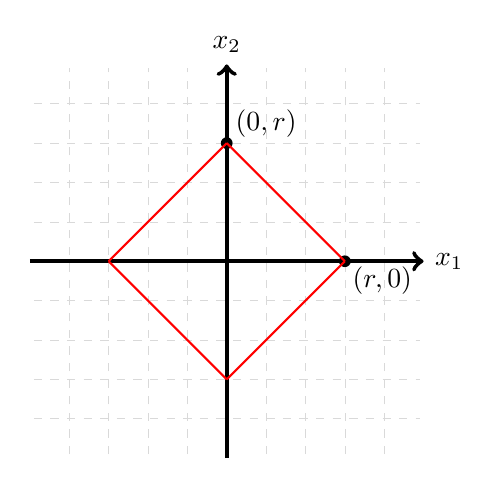
\begin{tikzpicture}[scale=0.5]
    \draw[help lines, color=gray!30, dashed] (-4.9,-4.9) grid (4.9,4.9);
    \draw[->,ultra thick] (-5,0)--(5,0) node[right]{$x_1$};
    \draw[->,ultra thick] (0,-5)--(0,5) node[above]{$x_2$};
    \node at (0,3) [circle,fill,inner sep=1.5pt]{};
    \node at (3,0) [circle,fill,inner sep=1.5pt]{};
    \node at (3.95,-0.5) {$(r,0)$};
    \node at (1,3.5) {$(0,r)$};
    
    \draw[-, thick, color=red] (3,0)--(0,3);
    \draw[-, thick, color=red] (-3,0)--(0,-3);
    \draw[-, thick, color=red] (-3,0)--(0,3);
    \draw[-, thick, color=red] (3,0)--(0,-3);
    \end{tikzpicture}}
    \subfloat[2-norm (Euclidean metric)]{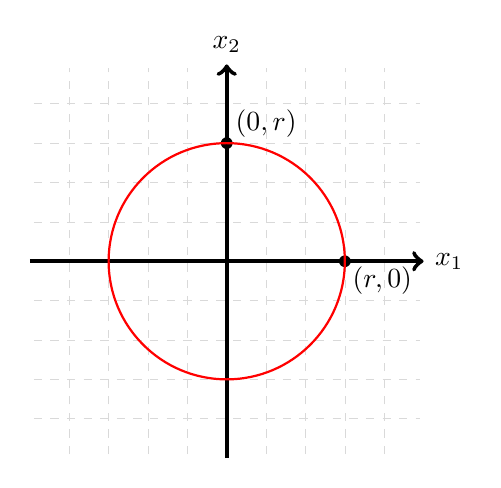
\begin{tikzpicture}[scale=0.5]
    \draw[help lines, color=gray!30, dashed] (-4.9,-4.9) grid (4.9,4.9);
    \draw[->,ultra thick] (-5,0)--(5,0) node[right]{$x_1$};
    \draw[->,ultra thick] (0,-5)--(0,5) node[above]{$x_2$};
    \node at (0,3) [circle,fill,inner sep=1.5pt]{};
    \node at (3,0) [circle,fill,inner sep=1.5pt]{};
    \node at (3.95,-0.5) {$(r,0)$};
    \node at (1,3.5) {$(0,r)$};
    
    \draw[thick, color = red] (0,0) circle [radius=3];
    \end{tikzpicture}}
    \subfloat[$\infty$-norm]{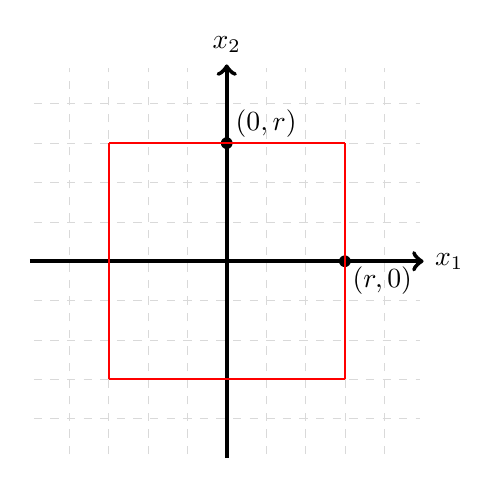
\begin{tikzpicture}[scale=0.5]
    \draw[help lines, color=gray!30, dashed] (-4.9,-4.9) grid (4.9,4.9);
    \draw[->,ultra thick] (-5,0)--(5,0) node[right]{$x_1$};
    \draw[->,ultra thick] (0,-5)--(0,5) node[above]{$x_2$};
    \node at (0,3) [circle,fill,inner sep=1.5pt]{};
    \node at (3,0) [circle,fill,inner sep=1.5pt]{};
    \node at (3.95,-0.5) {$(r,0)$};
    \node at (1,3.5) {$(0,r)$};
    
    \draw[-, thick, color=red] (3,-3) --(3,3);
    \draw[-, thick, color=red] (3,3) --(-3,3);
    \draw[-, thick, color=red] (-3,-3) --(-3,3);
    \draw[-, thick, color=red] (3,-3) --(-3,-3);
    \end{tikzpicture}}
    \caption{$B_r(0)$ for different metrics}
    \label{fig:open_ball}
\end{figure}

\end{example}

\begin{definition}[Open and closed sets]
Let $(X,d)$ be a metric space. 
\begin{itemize}
    \item A set $U \subseteq X$ is \emph{open} if for every $x \in U$ there exists $\epsilon>0$ such that $B_\epsilon(x) \subseteq U$.
    \item A set $K \subseteq X$ is \emph{closed} if $K^c:= X\setminus K$ is open.
\end{itemize}
\end{definition}

We note that $\emptyset$ and $X$ are both open and closed! 

\begin{proposition}
\label{prop:open_sets}
Let $(X,d)$ be a metric space. 
 \begin{enumerate}
     \item[(i)] Let $A_1,A_2\subseteq X$. If $A_1$ and $A_2$ are open, then $A_1 \cap A_2$ is open.
     \item[(ii)] If $A_i \subseteq X$, $i \in I$ are open, then $\cup_{i\in I} A_i$ is open.
 \end{enumerate}
\end{proposition}
\begin{proof}
(i) Since $A_1$ is open, for each $x \in A_1$, there exists an $\epsilon_1 > 0$ such that $B_{\epsilon_1}(x) \subseteq  A_1$. Since $A_2$ is open, for each $x \in A_2$, there exists an $\epsilon_2 > 0$ such that $B_{\epsilon_2}(x) \subseteq A_2$. Let $x \in A_1 \cap A_2$. Choose $\epsilon = \min\{\epsilon_1,\epsilon_2\}$. Then  $B_{\epsilon}(x) \subseteq A_1 \cap A_2$ as required. 

\vspace{1em}

(i) Let $x\in \cup_{i\in I} A_i$. Then there exists $i \in I$ such that $x \in A_i$, and since $A_i$ is open there exists $\epsilon>0$ such that $B_\epsilon(x) \subseteq  A_i$. Since $A_i \subseteq \cup_{i\in I} A_i$, we are done.

\end{proof}

We immediately have the following corollary:
\begin{corollary}
\label{cor:closed_sets}
Let $(X,d)$ be a metric space. 
 \begin{enumerate}
     \item[(i)] Let $A_1,A_2\subseteq X$. If $A_1$ and $A_2$ are closed, then $A_1 \cup A_2$ is closed.
     \item If $A_i \subseteq X$, $i \in I$ are closed, then $\cap_{i\in I} A_i$ is closed.
 \end{enumerate}
\end{corollary}

\begin{definition}[Interior and closure]
Let $A\subseteq X$ where $(X,d)$ is a metric space. 
\begin{itemize}
    \item The \emph{closure} of $A$ is  $\overline A :=\{x \in A: \forall \epsilon > 0 \; B_\epsilon(x) \cap A \neq \emptyset \}$
    \item The \emph{interior} of $A$ is  $\interior A :=\{x \in A: \exists \epsilon > 0 \text{ s.t. } B_\epsilon(x) \subseteq A \}$
    \item The \emph{boundary} of $A$ is $\partial A := \{ a \in X: \forall \epsilon > 0, \, B_\epsilon(x) \cap A \neq \emptyset \text{ and }  B_\epsilon(x) \cap A^c \neq \emptyset\}$
\end{itemize}
\end{definition}
The closure of a set is the smallest closed set that contains it while the interior of a set is the largest open set contained by it.

\begin{proposition}
 Let $A\subseteq X$ where $(X,d)$ is a metric space. Then $\interior A = A \setminus \partial A$.
\end{proposition}
\begin{proof}
First, we show $\interior A\subseteq A \setminus \partial A$. Let $x \in \interior A$. Then by definition $\exists \epsilon > 0 \text{ s.t. } B_\epsilon(x) \subseteq A$. Clearly $x \ A$ and also by definition, $x \notin \partial A$.

\vspace{1em}

Next, we show $A \setminus \partial A \subseteq \interior A$. Let $x \in A \setminus \partial A$. Then $x \in A$ and $x \notin \partial A$. The latter means that $\exists \epsilon > 0$ such that $B_\epsilon(x) \cap A \neq \emptyset$ or  $B_\epsilon(x) \cap A^c \neq \emptyset$. Since $x \in B_\epsilon(x) \cap A$ for any $\epsilon$, the former cannot be true for any $\epsilon$. Therefore $\exists \epsilon > 0$ such that $B_\epsilon(x) \cap A^c \neq \emptyset$, i.e. $B_\epsilon(x) \subseteq A$. Thus $x \in \interior A$.
\end{proof}

\begin{definition}
A subset $A$ of a metric space $(X,d)$ is \emph{bounded} if there exists $M>0$ such that $d(x,y) < M$ for all $x,y \in A$. 
\end{definition}


\subsection{Sequences}

\begin{definition}
Let $(X,d)$ be a metric space. A \emph{sequence} is a list of points $x_n$, $n\in\N$, in $X$, denoted $(x_n)_{n \in \N}$. We say that a sequence $(x_n)_{n \in \N}$ \emph{converges} to a point $x \in X$ if 
\begin{equation*}
    \forall \epsilon > 0 \, \exists \, n_\epsilon \in \N \text{ s.t. } d(x_n,x) < \epsilon \text{ for all } n \geq n_\epsilon .
\end{equation*}
\end{definition}

\begin{proposition}
\label{prop:closure_limit}
Let $(X, d)$ be a metric space, and let $A \subseteq X$. Then $\overline A$ is equal to the set of points in $X$ which are limits of a sequence in $A$.
\end{proposition}

\begin{proof}
Let $x \in \overline A$. Then by definition, for every $\epsilon > 0$, $B_\epsilon(x) \cap A \neq \emptyset$. In particular this is true for $\epsilon = 1/n$. Thus, for any $n \in N$, we can choose an $x_n \in A$ such that $x_n \in B_{1/n}(x)$, which means $d(x,x_n) < \frac{1}{n}$ by the definition of an open ball. Since $1/n$ decreases monotonically to zero, we must have $x_n \to x$.

Let $x \in X$ be the limit of a sequence $(x_n)_{n \in \N} \in A$. Then for $\epsilon > 0$, $\exists \, n_\epsilon \in \N$ such that $d(x_n,x) < \epsilon$ for all $n \geq n_\epsilon$. This means there $x_n \in B_\epsilon(x)$, and since $x_n \in A$, $B_\epsilon(x) \cap A \neq \emptyset$. Thus $x \in \overline A$.
\end{proof}

\begin{corollary}
\label{cor:closed_converge}
A set $K \subseteq X$, where $(X, d)$ is a metric space, is closed if and only if every sequence in $K$ which converges in $X$ converges to a point in $K$.
\end{corollary}

We also define a concept related to the closure of a set: a cluster or accumulation point.

\begin{definition}
Let $(X,d)$ be a metric space and $A \subseteq X$. A point $x \in X$ is a \emph{cluster point}of $A$ (also called accumulation point) if for every $\epsilon >0$, $B_\epsilon(x)$ contains uncountably many points in $A$.
\end{definition}

The following result also follows from \cref{prop:closure_limit}.

\begin{corollary}
 $x \in X$ is a cluster point of $A \subseteq X$ where $(X,d)$ is a metric space if and only if there exists a sequence of points $x_n \in A$, $n \in \N$, such that $x_n \to x$.
\end{corollary}

\begin{proposition}
For $A \subseteq X$, $(X,d)$ a metric space, we have $\overline{A} = A \cup \{x \in X : x \text{ is a cluster point of }A \}$.
\end{proposition}


\subsubsection{Cauchy sequences}

\begin{definition}[Cauchy sequence]
Let $(X,d)$ be a metric space. A sequence denoted $(x_n)_{n \in \N} \in X$ is called a \emph{Cauchy sequence} if
\begin{equation*}
    \forall \epsilon \, \exists \, n_\epsilon \in \N \text{ s.t. } d(x_n,x_m) < \epsilon \text{ for all } n,m \geq n_\epsilon .
\end{equation*}
\end{definition}

\begin{proposition}
\label{prop:converge_means_Cauchy}
Let $(X, d)$ be a metric space, and let $(x_n)_{n\in\N}$ be a convergent sequence in $X$. The  $(x_n)_{n\in\N}$ is Cauchy.
\end{proposition}

\begin{proof}
Let $\epsilon > 0$ be arbitrary. Let $(x_n)_{n\in\N}$ be a convergent sequence in a metric space $(X,d)$. Then there exists $n_\epsilon \in \N$ such that $d(x_n,x) < \frac{\epsilon}{2}$ for all $n \geq n_\epsilon$. Then for $n,m \geq n_\epsilon$, using the triangle inequality we have
\begin{equation*}
    d(x_n,x_m) \leq  d(x_n,x) +  d(x,x_m) < \frac{\epsilon}{2} + \frac{\epsilon}{2} = \epsilon .
\end{equation*}
Thus $(x_n)_{n\in\N}$ is Cauchy.
\end{proof}

\begin{definition}
A metric space where every Cauchy sequence converges (to a point in the space) is called \emph{complete}.
\end{definition}

In addition, a normed space that is complete with respect to the metric induced by the norm is called a \emph{Banach space}. $\R^n$ with the Euclidean distance is complete (and is in fact a Banach space). 

\begin{proposition}[{\cite[Proposition 2.4.5]{tastetopology}}]
\label{prop:closed_subset_complete}
Let $(X, d)$ be a metric space, and let $Y\subseteq X$.
\begin{enumerate}
    \item[(i)] If $X$ is complete and if $Y$ is closed in $X$, then $Y$ is complete.
    \item[(ii)] If $Y$ is complete, then it is closed in $X$.
\end{enumerate}
\end{proposition}

\begin{proof}
(i) Let $X$ be a complete metric space and $Y$ be a closed subset of $X$. Let $(x_n)_{n\in\N}$ be a Cauchy sequence in $Y$. Since $Y \subseteq X$, $(x_n)_{n\in\N}$ is also a Cauchy sequence in $X$. Therefore $(x_n)_{n\in\N}$ converges to an $x \in X$ since $X$ is complete. But since $Y$ is closed, by \cref{prop:closure_limit}, we must have $x \in Y$. Therefore $Y$ is complete.

(ii) Let $(X, d)$ be a metric space and let $Y\subseteq X$ be complete. Let $(y_n)_{n\in\N}$ be a sequence in $Y$ that converges to some point $y \in X$.  By \cref{prop:converge_means_Cauchy},  $(y_n)_{n\in\N}$ is Cauchy in $X$ and therefore also in $Y$. Since $Y$ is complete, $(y_n)_{n\in\N}$ converges to a point $y' \in Y$. Since sequences in metric spaces converge to unique points (\cref{exercises:metric_spaces}, exercise 6), $y=y'$. Thus $Y$ is closed by \cref{cor:closed_converge}.
\end{proof}

\subsubsection{Subsequences}

\begin{definition}
Let $(x_n)_{n \in \N}$ be a sequence in a metric space $(X,d)$. Let $(n_k)_{k \in \N}$ be a sequence of natural numbers with $n_1 < n_2 < \cdots$. The sequence $(x_{n_k})_{k \in \N}$ is called a \emph{subsequence} of $(x_n)_{n \in \N}$. If $(x_{n_k})_{k \in \N}$ converges to $x \in X$, we call $x$ a \emph{subsequential limit}.
\end{definition}

\begin{example}
The sequence $\left((-1)^n\right)_{n \in \N}$ diverges but the subsequences $\left((-1)^{2n}\right)_{n \in \N}$ and $\left((-1)^{2n-1}\right)_{n\in \N}$ converge to subsequential limit points 1 and $-1$, respectively.
\end{example}

\begin{proposition}
A sequence $(x_n)_{n \in \N}$ in a metric space $(X,d)$ converges to $x \in X$ if and only if every subsequence of $(x_n)_{n \in \N}$  also converges to $x$.
\end{proposition}
\begin{proof}
($\Leftarrow$) If every subsequence of $(x_n)_{n \in \N}$ converges to $x \in X$, then  $(x_n)_{n \in \N}$ must converge to it as well, since a sequence is a subsequence of itself. 

($\Rightarrow$) Suppose $(x_n)_{n \in \N}$ converges to $x \in X$ and let $(x_{n_k})_{k \in \N}$ be an arbitrary subsequence of $(x_n)_{n \in \N}$. Let $\epsilon > 0$ be arbitrary. There exists $n_\epsilon \in \N$ such that $d(x_n,x) < \epsilon$ for all $n \geq n_\epsilon$. Choose $k_\epsilon$ such that $n_{k_\epsilon} \geq n_\epsilon$, which must exist since $(n_k)_{k\in\N}$ is strictly increasing. Then for all $k \geq k_\epsilon$, $d(x_{n_k},x) < \epsilon$. Thus $(x_{n_k})_{k \in \N}$ converges to $x$.
\end{proof}


\subsection{Continuity}

\begin{definition}
Let $(X,d_X)$ and $(Y,d_Y)$ be metric spaces, let $x_0 \in X$, and let $f:X\to Y$. $f$ is \emph{continuous} at $x_0$ if for every sequence $(x_n)_{n\in\N}$ in $X$ that converges to $x_0$, we have $\lim_{n\to\infty}f(x_n)=f(x_0)$.
We say that $f$ is continuous if it is continuous at every point in $X$.
\end{definition}

\begin{theorem}[{\cite[Theorem 2.3.7.]{tastetopology}}]
\label{thm:cont_equiv}
Let $(X,d_X)$ and $(Y,d_Y)$ be metric spaces, let $x_0 \in X$, and let $f:X\to Y$. The following are equivalent:
\begin{enumerate}
    \item[(i)] $f$ is continuous at $x_0$
    \item[(ii)] for all $\epsilon>0$, there exists $\delta > 0$ such that $d_Y(f(x),f(x_0))) < \epsilon$ for all $x \in X$ with $d_X(x,x_0) < \delta$
    \item[(iii)] for each $\epsilon>0$, there is $\delta > 0$ such that $B_\delta(x_0) \subseteq f^\inv (B_\epsilon(f(x_0)))$
\end{enumerate}
\end{theorem}

\begin{proof}
(i) $\Rightarrow$ (ii) We prove the contrapositive. Assume
\begin{equation}
\label{star1} 
\exists \epsilon_0 \text{ such that } \forall \delta > 0 \text{ there exists an } x_\delta \in X \text{ with } d_X(x_\delta,x_0) < \delta \text{ and } d_Y(f(x_\delta),f(x_0))) \geq \epsilon_0
\tag{$\star$}
\end{equation}
We need to find a sequence in $X$ that converges to  $x_0$ but the sequence of images does not converge. Let's construct such a sequence. 

Let $\delta=\frac{1}{n}$ in \eqref{star1} for $n \in \N$. Then we have a sequence $x_n := x_{1/n}$ given by \eqref{star1} which converges to $x_0$. However, for each $n \in \N$, we have $d_Y(f(x_n),f(x_0))) \geq \epsilon_0$, so we cannot have $\lim_{n\to\infty}f(x_n)=f(x_0)$.

\vspace{1em}

(ii) $\Rightarrow$ (iii) Follows from the definitions of the pre-image and open balls. 

\vspace{1em}

(iii) $\Rightarrow$ (i) Let $(x_n)_{n\in\N}$ be a sequence in $X$ that converges to $x_0$. Let $\epsilon > 0$. Then by (iii), there exists $\delta > 0$ such that $B_\delta(x_0) \subseteq f^\inv (B_\epsilon(f(x_0)))$, i.e. if $x$ is such that $d_X(x,x_0) < \delta$, then $x$ is such that  $d_Y(f(x),f(x_0)) < \epsilon$. By the definition of convergence, there exists a $N \in \N$ such that $d(x_n,x_0)< \delta$ for all $n \geq N$. Then by(iii), $d(f(x_n),f(x_0))< \epsilon$ for all $n \geq N$. Thus $\lim_{n\to\infty}f(x_n)=f(x_0)$.

\end{proof}

\begin{corollary}
Let $(X,d_X)$ and $(Y,d_Y)$ be metric spaces and let $f:X\to Y$. The following are equivalent:
\begin{enumerate}
    \item[(i)] $f$ is continuous
    \item[(ii)] if $U \subseteq Y$ is open, then $f^\inv(U)$ is open
    \item[(iii)] if $F \subseteq Y$ is closed, then $f^\inv(F)$ is closed
\end{enumerate}
\end{corollary}

\textit{Note: the following proof uses the following results, which you may wish to prove as an exercise using techniques from the set theory section if they are not clear to you: Let $X$ and $Y$ be sets and $f:X \to Y$. Let $A,B \subseteq Y$. Then 
\begin{enumerate}
\item $f^\inv(A) \subseteq f^\inv(B)$
\item $f^\inv(Y \setminus A) = X \setminus f^\inv(A)$
\end{enumerate}}

\begin{proof}
Let $(X,d_X)$ and $(Y,d_Y)$ be metric spaces and let $f:X\to Y$.

\vspace{1em}

(i) $\Rightarrow$ (ii): Suppose $f$ is continuous (on every point in $X$) and let $U \subseteq Y$ be open. Let $x \in f^\inv(U)$, then $f(x) \in U$, and since $U$ is open, there exists $\epsilon_0 > 0$ such that $B_{\epsilon_0}(f(x)) \subseteq U$. By \cref{thm:cont_equiv}(iii), there exists a $\delta_0$ such that $B_{\delta_0}(x) \subseteq f^\inv (B_{\epsilon_0}(f(x)))$. Since $B_{\epsilon_0}(f(x))) \subseteq U$, $f^\inv (B_{\epsilon_0}(f(x))) \subseteq f^\inv(U)$. Thus for each $x \in f^\inv(U)$, there exists $\delta_0$ such that $B_{\delta_0}(x) \subseteq f^\inv (B_{\epsilon_0}(f(x))) \subseteq f^\inv(U)$, so $f^\inv(U)$ is open.

\vspace{1em}

(ii) $\Rightarrow$ (i): We want to prove that $f$ is continuous at every $x \in X$ using the definition from \cref{thm:cont_equiv}(iii), i.e. we must show that for $x \in X$, for each $\epsilon>0$, there is $\delta > 0$ such that $B_\delta(x) \subseteq f^\inv (B_\epsilon(f(x)))$. 

Let $x\in X$ and let $\epsilon > 0$ be arbitrary. Since $B_\epsilon(f(x))$ is an open set, by (ii), $f^\inv(B_\epsilon(f(x)))$ is also open. Since $x \in f^\inv(B_\epsilon(f(x)))$, there exists a $\delta > 0$ such that $B_\delta(x) \subseteq f^\inv(B_\epsilon(f(x)))$ by the definition of a set being open, so we are done.

\vspace{1em}


(ii) $\Rightarrow$ (iii): Let $F \subseteq Y$ be closed. Then $Y \setminus F$ is open, so by (ii), $f^\inv(Y \setminus F)$ is open as well. Since $f^\inv(Y \setminus F) = X\setminus f^\inv(F)$, $f^\inv(F)$ is closed.

\vspace{1em} 

(iii) $\Rightarrow$ (ii) follows from the above, exchanging ``open'' and ``closed''.

\end{proof}



\begin{definition}
Let $(X,d_X)$ and $(Y,d_Y)$ be metric spaces and let $f:X\to Y$. 
\begin{itemize}
    \item $f$ is \emph{uniformly continuous} if for all $\epsilon>0$, there exists $\delta > 0$ such that for every $x_1,x_2\in X$ with $d_X(x_1,x_2) < \delta$, we have  $d_Y(f(x_1),f(x_2))) < \epsilon$ 
    \item $f$ is \emph{Lipschitz continuous} if there exists a $K > 0$ such that for every $x_1,x_2\in X$ we have  $d_Y(f(x_1),f(x_2))) < K d_X(x_1,x_2)$
\end{itemize}
\end{definition}

\begin{proposition}
Let $(X,d_X)$ and $(Y,d_Y)$ be metric spaces and let $f:X\to Y$. 
$$f \text{ is Lipschitz continuous } \Rightarrow \text{ f is uniformly continuous } \Rightarrow \text{ f is continuous}$$
\end{proposition}

The proof is left as an exercise. 

\begin{definition}
Let $(X,d)$ be a metric space and let $f:X \to X$. We say that $x^* \in X$ is a \emph{fixed point} of $f$ if $f(x^*) = x^*$.
\end{definition}

\begin{definition}
Let $(X,d)$ be a metric space and let $f:X \to X$. $f$ is a \emph{contraction} if there exists a constant $k \in [0,1)$ such that for all $x,y \in X$, $d(f(x),f(y))) \leq k d(x,y)$.
\end{definition}

Observe that a function is a contraction iff it is Lipschitz continuous with constant $K < 1$.

\begin{theorem}
Suppose that $f : X \to X$ is a contraction and the metric space $X$ is complete. Then $f$ has a unique fixed point $x^*$.
\end{theorem}

We omit the proof here; see \cite[p.240]{realanalysis} for the proof as well as more details on how to find the fixed point.

\begin{example}
Let $f:\left[-\frac{1}{3},\frac{1}{3}\right] \to \left[-\frac{1}{3},\frac{1}{3}\right]$ be defined by the mapping $x \mapsto x^2$. Assume we use the standard Euclidean metric, $d(x,y) = |x-y|$. $f$ has a unique fixed point because $\left[-\frac{1}{3},\frac{1}{3}\right]$ is a complete metric space (see \cref{prop:closed_subset_complete}) and $f$ is a contraction with Lipschitz constant 2/3.

To see that it is a contraction, let $x,y \in \left[-\frac{1}{3},\frac{1}{3}\right]$. Then
\begin{equation*}
   |x^2 - y^2| = |x+y| |x-y| \leq \frac{2}{3} |x-y|. 
\end{equation*}
\end{example}

\subsection{Equivalence of metrics}

\begin{definition}[Equivalent metrics]
Two metrics $d_1$ and $d_2$ on a set $X$ are \emph{equivalent} if the identity maps from $(X,d_1)$ to $(X,d_2)$ and from $(X,d_2)$ to $(X,d_1)$ are continuous. 
\end{definition}

\begin{proposition}
Two metrics $d_1$, $d_2$ on a set $X$ are equivalent iff they have the same open sets or the same closed sets.
\end{proposition}

\begin{definition}
Two metrics $d_1$ and $d_2$ on a set $X$ are \emph{strongly equivalent} if for every $x,y\in X$, there exists constants $\alpha>0$ and $\beta>0$ such
\begin{equation*}
    \alpha d_1(x,y) \leq d_2(x,y) \leq \beta d_1(x,y).
\end{equation*}
\end{definition}

If two metrics are strongly equivalent then they are equivalent. The proof of this is one of the exercises. 

\begin{example}
We show that the Euclidean distance (induced by 2-norm) and the metric induced by the $\infty$-norm are equivalent on $\R^n$. 

\vspace{1em}
Let $||x-y||_2=\sqrt{\sum_{j=1}^n (x_j - y_j)^2}$ be the Euclidean metric and $||x-y||_\infty= \max_{j=1,\ldots,n} |x_j - y_j|$ be the $\infty$-norm metric. We have
\begin{equation*}
   ||x-y||_2 = \sqrt{\sum_{j=1}^n (x_j - y_j)^2} \leq  \sqrt{ n \max_{j=1,\ldots,n} (x_j - y_j)^2}  = \sqrt{n} \max_{j=1,\ldots,n} |x_j - y_j| = \sqrt{n} \, ||x-y||_\infty
\end{equation*}
and
\begin{equation*}
    ||x-y||_\infty = \max_{j=1,\ldots,n} |x_j - y_j|  = \sqrt{\max_{j=1,\ldots,n} (x_j - y_j)^2} \leq \sqrt{\sum_{j=1}^n(x_j - y_j)^2}  = ||x-y||_2  \, .
\end{equation*}
Thus the two metrics are strongly equivalent. 
\end{example}

\subsection{Extra properties of $\R^n$}


\emma{left- and right- continuous on $\R$, \\
series, Conditional and absolute convergence, Convergence tests \\
sup, inf lim sup, lim inf, sup norm?}

\subsection{Exercises}
\label{exercises:metric_spaces}
\begin{enumerate}
    \item Show that the infinity norm $||x||_\infty$, $x \in \R^n$, defined in \cref{p-norm} is a norm.
    \item Let $(X,d)$ be any metric space, and define $\tilde d: X \times X \to \R$ by 
    \begin{equation*}
        \tilde d(x,y) = \frac{d(x,y)}{1+d(x,y)}, \quad x,y \in X .
    \end{equation*}
    Show that $\tilde d$ is a metric on $X$.
    \item Let $X$ be a set and define $d\colon X \times X \to \R$ by $d(x,x) = 0$ and $d(x,y)=1$ for $x\neq y \in X$. Prove that $d$ is a metric on $X$. What do open balls look like for different radii $r>0$? What does an arbitrary open set look like?
    \item Following up on \cref{prop:open_sets} and \cref{cor:closed_sets}: Show that the infinite intersection of open sets may not be open and that the infinite union of closed sets may not be closed.
    \item Find the closure, interior, and boundary of the following sets using Euclidean distance:
    \begin{enumerate}
        \item[(i)] $\{(x,y)\in \R^2 : y < x^2 \} \subseteq \R^2$
        \item[(ii)]  $[0,1)\times[0,1) \subseteq \R^2$
        \item[(iii)] $\{0 \} \cup  \{1/n \colon n \in \N\} \subseteq \R$ 
    \end{enumerate}
    \item Prove the following: Let $(x_n)_{n\in\N}$ be a sequence in a metric space $(X,d)$ that converges to a point $x \in X$. Then $x$ is unique.
    \item Prove the following: Let $(x_n)_{n \in \N}$ and $(y_n)_{n \in \N}$ be sequences in $\R$ such that $x_n \to x$ and and $y_n \to y$, with $\alpha, x,y, \in \R$. 
    \begin{enumerate}
        \item[(i)] Show that $\alpha \, x_n \to \alpha \, x$.
        \item[(i)] Show that $x_n + y_n \to x + y$.
    \end{enumerate}
    \item Show that discrete metric spaces (i.e. those with the metric from exercise 3) are complete. 
    \item Let $(X,d_X)$ and $(Y,d_Y)$ be metric spaces and let $f:X\to Y$. Prove that
$$f \text{ is Lipschitz continuous } \Rightarrow f \text{ is uniformly continuous } \Rightarrow f \text{ is continuous}.$$
Provide examples to show that the other directions does not hold.
    \item Show that the function $f(x) = \frac{1}{2} \left(x + \frac{5}{x} \right)$ has a unique fixed point on $(0,\infty)$. What is it? (Hint: you will have to restrict the interval.)
    \item Prove the following: If two metrics are strongly equivalent then they are equivalent. 
\end{enumerate}

\subsection{References}
The content in this section comes following texts:

A Taste of Topology \cite{tastetopology} \\
Real Mathematical Analysis \cite{realanalysis} \\
The first chapter of Piotr Zwiernik's  \textit{Lecture notes in Mathematics for Economics and Statistics} \cite{piotr}


\section{Topology}

\subsection{Basic definitions}

Let $X$ be a set. If $X$ is not a metric space, can we still have open and closed sets? This motivates the concept of a topology. One can think of a topology on $X$ as a specification what subsets of $X$ are open. From the previous section (metric spaces), we already saw some properties of open and closed sets. This motivates the following definition. 

\begin{definition}
Let $\cT\subseteq \cP(X)$. We call $\cT$ a \emph{topology} on $X$ if the following holds:
\begin{itemize}
    \item[(i)] $\emptyset, X \in \cT$
    \item[(ii)] If $\{U_\alpha\}_{\alpha \in A }\subseteq \cT$, then $\bigcup_{\alpha \in A} U_\alpha \in \cT$ ($\cT$ is closed under arbitrary unions)
    \item[(iii)] Let $n \in \N$. If $U_1, \ldots, U_n \in \cT$, then $\bigcap_{i=1}^n U_i \in \cT$ ($\cT$ is closed under finite intersections)
\end{itemize}
If $U\in \cT$, we call $U$ \emph{open}. We call $U\subseteq X$ \emph{closed}, if $U^c\in \cT$. We call $(X,\cT)$ a \emph{topological space}.
\end{definition}

Alternatively we could have specified closed sets, and obtained similar axioms using De Morgan's rules. 

\begin{example}
For a set $X$, the following $\cT \subseteq \cP(X)$ are examples of topologies on $X$.
\begin{itemize}
    \item Trivial topology: $\cT = \{\emptyset, X\}$,
    \item Discrete topology: $\cT=\cP(X)$,
    \item Topology induced by metric: i.e. if $d$ is a metric on $X$ we can define 
    $$\cT_d = \{U \subseteq X \; \vert \; \forall x \in U \, \exists \epsilon>0 \text{ such that } B_\epsilon(x) \subseteq U \}.$$
    The discrete topology is also induced by a metric, can you guess which one?
    \item $\cT = \{U \subseteq X \;\colon\; U^c \; \text{is finite}\}\cup \emptyset$
\end{itemize}
\end{example}

Given a topological space $(X,\cT)$ and a subset $Y\subseteq X$ we can restrict the topology on $X$ to $Y$ which leads to the next definition. 

\begin{definition}[Relative topology]
Given a topological space $(X,\cT)$ and an arbitrary non-empty subset $Y \subseteq X$, we define the relative topology on $Y$ as follows
\begin{equation*}
    \cT\vert_Y = \{U\cap Y \; \colon\; U \in \cT\}.
\end{equation*}
\end{definition}

Recall that in the metric space setting, we had set theoretic descriptions of closures and interiors of sets. We will generalize this in the next definition.

\begin{definition}
Let $(X,\cT)$ be a topological space and let $A\subseteq X$ be any subset.
\begin{itemize}
    \item The \emph{interior} of $A$ is $\interior A := \{a \in A \colon \exists U \in  \cT \text{ s.t. } U\subseteq A \text{ and } a\in U\} $.
    \item The \emph{closure} of $A$ is $\overline{A} := \{x \in X \colon \forall U \in \cT \text{ with } x \in U, U\cap A \neq \emptyset\}$.
    \item The \emph{boundary} of $A$ is $\partial A:= \{x \in X \colon \forall U\in \cT \text{ with } x\in U, U \cap A \neq \emptyset \text{ and } U \cap A^c \neq \emptyset \}$.
\end{itemize}
\end{definition}
One can see that the definitions are taken fairly verbatim from the metric space setting, except that we are now looking at arbitrary open sets given by the topology instead of balls of the form $B_\epsilon(x)$. Similar to the metric space setting, the interior is the largest open set contained in $A$, whereas the the closure is the smallest closed set that contains $A$. 

\begin{example}
Let $X=\{a,b,c\}$ and $\cT = \{\emptyset ,\{a\}, \{b\},\{a,b\}, X\}$. Then the following holds
\begin{itemize}
    \item $ \interior{\{ a\} }= \{a\}$,
    \item $\interior{ \{c\}} = \emptyset$,
    \item $\overline{\{a\}} = \{a,c\}$,
    \item $\overline{\{c\}} = \{c\}$.
\end{itemize}
\end{example}

Note that even though we do not necessarily have a characterization of closures in terms of limits of sequences as in metric spaces for arbitrary topological spaces, there exists an alternative characterization that still holds in this general setting (and thus in particular also for metric spaces).

\begin{proposition}[Proposition 3.1.18 in \cite{tastetopology}]
 Let $(X,\cT)$ be a topological space and $A\subseteq X$. Then,
 \begin{equation*}
     \overline{A} = \bigcap \{F \colon F \text{ is closed and } A \subseteq F\}.
 \end{equation*}
\end{proposition}
\begin{proof}
For convenience define $A^\prime = \bigcap \{F \colon F \text{ is closed and } A \subseteq F\}$. We will show $ \overline{A}\subseteq A^\prime$ by showing that $(A^\prime)^c \subseteq \overline{A}^c$ (contrapositive). Suppose $x\not \in A^\prime$. Then, since the closure is closed, $(A^\prime)^c$ is an open set containing $x$. But since $A \subseteq A^\prime$ we have $A\cap (A^\prime)^c = \emptyset$, showing that $x\not \in \overline{A}$. 

Conversely, assume $X\not \in \overline{A}$. Then there exists an open set $U$ with $x\in U$ such that $U\cap A = \emptyset$. Thus, $A\subseteq U^c$. Since $U^c$ is closed, we have by the definition of closure $A^\prime \subseteq U^c$ and since $x\not \in U^c$, we have $x\not \in A^\prime$. Thus, $A^\prime\subseteq \overline{A}$.
\end{proof}

Similarly, one can show $\interior A =\bigcup \{U: U \text{ is open and } U \subseteq A \}$. Hence, we see that the interior of $A$ is the largest open set contained in $A$ and the closure is the smallest closed set that contains $A$.

\vspace{1em}

Another important concept in topology (and thus also in metric spaces) is density. 

\begin{definition}
Let $(X,\cT)$ be a topological space. A subset $A\subseteq X$ is called \emph{dense}, if $\overline{A} = X$ 
\end{definition}

Using the definition of closure, we see that $A\subseteq X$ is dense if and only if for all $U\in \cT$, $U\cap A \neq \emptyset$.

\begin{example}
\textcolor{white}{Skip}
\begin{itemize}
    \item The rationals $\Q$ are dense in the reals $\R$. 
    \item The only dense subset in $(X,\cP(X))$ is $X$ itself.
    \item Any non-empty subset is dense in $(X,\{\emptyset,X\})$.
\end{itemize}
\end{example}

The concept of a dense subset allows us to look at it instead of the whole space. In the metric space setting, this means that elements in $X$ can be approximated arbitrarilyw well with elements from the dense subset.

\begin{definition}
A topological space $(X,\cT)$ is \emph{separable} if there exists a countable dense subset.
\end{definition}

As stated in the previous example the rationals are dense in $\R$, and since $\Q$ is countable, $\R$ is separable. We could extend this example to $\R^n$. However, if we look at all bounded real-valued sequences with the metric induced by the supremums norm, this space fails to be countable. 

\begin{example}
Define $\ell_\infty=\{ (x_n)_{n\in \N} \, : x_n \in \R , \; \sup_{n\in \N} \vert x_n \vert <\infty \}$, the space of bounded real valued sequences. We can endow $\ell_\infty$ with a metric induced by the supremum norm, namely $d((x_n)_{n\in \N}, (y_n)_{n\in \N}) = \sup_{n\in \N} \vert x_n-y_n\vert$. Then $\ell_\infty$ is not separable with respect to the topology induced by this metric. To see this, for each $M\subseteq \N$ define 
\begin{equation*}
    e^M_n = \begin{cases} 1 \; \text{ if } n \in A,\\
    0 \; \text{ otherwise},
    \end{cases}
\end{equation*}
for $n \in \N$.  Then if $M_1, M_2\subseteq \N$ with $M_1\neq M_2$, $d((e^{M_1}_n)_{n\in \N},(e^{M_2}_n)_{n\in \N}) = 1$. Thus the open balls $B_{1/3}((e^{M_1}_n)_{n \in \N})$, $B_{1/3}((e^{M_2}_n)_{n \in \N})$ are disjoint for all $M_1, M_2\subseteq \N$ with $M_1\neq M_2$ (check using contradiction and triangle inequality). 

Now suppose towards contradiction $A \subseteq \ell^\infty$ is dense and countable.  Then by density, for all open sets $U$, $U\cap A \neq \emptyset$. In particular for all $M \subseteq \N$, $B_{1/3}((e^{M}_n)_{n \in \N})\cap A \neq \emptyset$. However, there are uncountably many such $M$ (see the cardinality of $\cP(\N)$ in the set theory section), but only countably many elements in $A$. Since the balls are disjoint, this is a contradiction. 
\end{example}


\subsection{Compactness}

We will start off by giving the definition of an important separation axiom. 

\begin{definition}
A topological space $(X,\cT)$ is called Hausdorff if for all $x\neq y\in X$ there exist open sets $U_x,U_y$ with $x\in U_x$ and $y\in U_y$ such that $U_x \cap U_y = \emptyset$.
\end{definition}

\begin{example}
\textcolor{white}{Skip}
\begin{itemize}
    \item Let $(X,d)$ be a metric space. Then $(X,\cT_d)$ is Hausdorff, where $\cT_d$ is the topology induced by the metric $d$. Why? If $x\neq y \in X$, then choose $\epsilon:= d(x,y)>0$ and thus $U_x=B_{\epsilon/2}(x)$ and $U_y=B_{\epsilon/2}(y)$ are disjoint. 
    \item Let $X$ be an infinite set and $\cT = \{U\subseteq X \colon U^c \text{ is finite } \}$. Then  $(X,\cT)$ is not Hausdorff. Why? Suppose in order to derive a contradiction that it is Hausdorff and take $x\neq y \in X$. Then there exist open sets $U_x,U_y$ with $x\in U_x$ and $y\in U_y$ such that $U_x \cap U_y = \emptyset$. However since $U_x \cap U_y$ is open, its complement $X$ is finite; a contradiction. 
\end{itemize} 
\end{example}

\begin{definition}
Let $(X,\cT)$ be a topological space and $K\subseteq X$. An collection $\{U_i\}_{i\in I}$ of open sets is called \emph{open cover} of $K$ if $K\subseteq \cup_{i\in I} U_i$. The set $K$ is called \emph{compact} if for all open covers $\{U_i\}_{i\in I}$ there exists a finite subcover, meaning there exits an $n\in \N$ and $\{U_1,\ldots,U_n\}\subseteq \{U_i\}_{i\in I}$ such that $K\subseteq \cup_{i=1}^n U_i$.
\end{definition}

\begin{proposition}[{\cite[Proposition 3.3.6]{tastetopology}}] Let $(X,\cT)$ be a topological space and take a non-empty subset $K\subseteq X$. The following holds:
\begin{enumerate}
    \item If $X$ is compact and $K$ is closed then $K$ is compact (i.e. closed subsets of compact sets are compact).
    \item If $(X,\cT)$ is Hausdorff, then $K$ being compact implies that $K$ is closed.
\end{enumerate}
\end{proposition}
\begin{proof}
1. We need to show that any open cover of $K$ has a finite subcover. Let $\{U_i\}_{i\in I}$ be an open cover of $K$. Then, since $K^c$ is open, $\{U_i\}_{i\in I} \cup {K^c}$ is an open cover of $X$. Since $X$ is compact there exists a finite subcover. There are two possibilities,  the finite subcover is either of the form $\{U_1, \ldots, U_n, K^c\}$ or $\{U_1, \ldots, U_n\}$. In either case, $\{U_1, \ldots, U_n\}$ is a finite subcover for $K$. Hence, $K$ is compact. 
    
2. We will show that $K^c$ is open. Let $x\in K^c$. Then, since $X$ is Hausdorff, for all $y\in K$ there exist disjoint open sets $U_{x,y}$ and $U_y$ with $x\in U_{x,y}, y\in U_y$. We would like to take the intersection over the $U_{x,y}$ to obtain an open set containing $x$ and contained in $K^c$ (note that the union would not work since we want to guarantee that the resulting set is still contained in $K^c$). However, since $K$ is compact and $\{U_y\}_{y\in K}$ is an open cover of $K$ there exist $y_1,\ldots, y_n$ such that $K\subseteq \cup_{i=1}^n U_{y_i}$. Thus $\tilde U = \cap_{i=1}^n U_{x,y_i}$ is open and $x\in \tilde U$ with $\tilde U \subseteq K^c$. Thus, $K^c$ is open. 
\end{proof}

In undergraduate math classes you may have seen an equivalent definition for compactness on $\R^n$. This is a nice feature of Euclidean space.

\begin{theorem}[Heine-Borel Theorem]
Let $K\subseteq \R^n$. Then $K$ is compact with respect to the topolgy induced by the Euclidean distance if and only if it is closed and bounded.
\end{theorem}

The proof is omitted. See \cite[Corollary 2.5.12]{tastetopology}.

\vspace{1em}

Just as we had a sequential characterization of the closure of a set in metric spaces, we similarly have a sequential characterization of compactness. 

\begin{theorem}
Let $(X,d)$ be a metric space. Then $K\subset X$ is compact with respect to the metric induced by $d$ if and only if every sequence in $K$ admits a subsequence converging to some point in $K$.
\end{theorem}

Again the proof is omitted. See \cite[Theorem 2.5.10]{tastetopology}. A corollary of this statement together with Heine-Borel is the Bolzano-Weierstrass theorem.

\begin{corollary}[Bolzano-Weierstrass]
Any bounded sequence in $\R^n$ has a convergent subsequence.
\end{corollary}

\subsection{Continuity}

Lastly, we will discuss continuity in this general setting. 

\begin{definition}
Let $(X,\cT_X)$ and $(Y,\cT_Y)$ be topological spaces. A map $f\colon X \to Y$ is called \emph{continuous} if for all $U\in \cT_Y$, $f^{-1}(U)\in \cT_X$, i.e. the preimage of open sets is open. 
\end{definition}

We can also specify continuity at a point $x_0\in X$.

\begin{definition}
Let $(X,\cT_X)$ and $(Y,\cT_Y)$ be topological spaces. A map $f\colon X \to Y$ is called \emph{continuous at $x_0\in X$} if for all $U\in \cT_Y$ with $f(x_0)\in U$, $f^{-1}(U)\in \cT_X$, i.e. the preimage of open sets containing $f(x_0)$ is open (and contains $x_0$).
\end{definition}

The next proposition is, in a certain sense, a generalization of the extreme value theorem to topological spaces.

\begin{proposition}
Let $(X,\cT_X)$ and $(Y, \cT_Y)$ be topological spaces. Suppose $K\subset X$ is compact and let $f\colon K \to Y$ be continuous. Then $f(K)$ is compact. 
\end{proposition}

\begin{proof}
Let $\{U_i\}_{i\in I}$ be an open cover of $f(K)$, i.e. $f(K) \subseteq \bigcup_{i\in I} U_i$. Then $f^{-1}(f(K)) \subseteq f^{-1}(\bigcup_{i\in I} U_i)$ (check!). By Exercise 6 in \cref{subsec:ex_set_theory}, we have $f^{-1}(\bigcup_{i\in I} U_i) = \bigcup_{i\in I}f^{-1} (U_i)$ and by \cref{prop:set_subset_preim_im}, we have $K\subseteq f^{-1}(f(K))$. Hence, we obtain $K \subseteq \bigcup_{i\in I}f^{-1} (U_i)$. Since $f$ is continuous, each $f^{-1} (U_i)$ is open and thus $\{f^{-1} (U_i)\}_{i\in I}$ is an open cover of $K$. Since $K$ is compact, there exist $f^{-1}(U_1),\ldots, f^{-1}(U_n)$ such that $K \subseteq \bigcup_{i=1}^n f^{-1}(U_i)$. Then $f(K) \subseteq f(\bigcup_{i=1}^n f^{-1}(U_i)) = \bigcup_{i=1}^n f(f^{-1}(U_i)) \subseteq \bigcup_{i=1}^n U_i$, where we use that images preserve set inclusions (check!), and Exercises 5 and 6 in \cref{subsec:ex_set_theory}. Thus, $\{U_1,\ldots, U_n\}$ is a finite subcover for $f(K)$ and $f(K)$ is compact. 
\end{proof}

As you can see, a lot of results from introductory real analysis or calculus have extensions to a more general topological setting. However, topology is a large field with many powerful tools that we do not have time to cover. The final result in this section is an important result in topology.

\begin{definition}
A topological space $(X,\cT)$ is \emph{normal} if the following hold:
\begin{itemize}
    \item[(i)] For all $x\in X$, $\{x\}$ is closed.
    \item[(ii)] For all  disjoint closed sets $F_1,F_2\subseteq X$ there exist disjoint open sets $U_1, U_2$ such that $F_1\subseteq U_1$ and $F_2\subseteq U_2$.
\end{itemize}
\end{definition}

\begin{example}
\textcolor{white}{Skip}
\begin{itemize}
    \item Any metric space $(X,d)$ is normal.
    \item Let $(X,\cT)$ be Hausdorff and compact. Then $X$ is normal.
    \item If $(X,\cT)$ is normal, then it is Hausdorff. 
\end{itemize}
\end{example}

\begin{theorem}[Urysohn's Lemma]
Let $(X,\cT)$ be normal and $F_1,F_2\subseteq X$ be closed with $F_1\cap F_2 = \emptyset$. Then there exists a continuous function $f\colon X \to [0,1]$ such that $f(F_1) = \{0\}$ and $f(F_2) = \{1\}$. (Here the topology on $[0,1]$ is the relative topology inherited from the usual metric topology on $\R$.)
\end{theorem}

Proof omitted. See \cite[Theorem 4.1.2]{tastetopology}.

\subsection{Exercises}
%Some theorems with open, closed sets as exercises (closure of union contains union of closures and equal in finite case closure of intersection is subset of intersection of closures, but might not be equal in any setting! counter example $A=[0,1), B=(1,0]$ then $\overline{A} \cap \overline{B} = \{1\}$, but $\overline{A\cap B}= \emptyset $) You can also do Chapter 3 Exercise 7 in \cite{tastetopology} if you want.
\begin{enumerate}
    \item Let $(X, \cT)$ be a topological space. Prove that $A\subseteq X$ is closed if and only if $\overline{A} =A$.
    \item Let $(X,\cT)$ be a topological space and $\{A_i\}_{i\in I}$ be a collection of subsets of $X$. Show that 
    \begin{equation*}
        \bigcup_{i\in I}\overline{A_i} \subseteq \overline{\bigcup_{i\in I}A_i}.
    \end{equation*}
    Show that if the collection is finite, the two sets are equal. 
    \item Let $(X,\cT)$ be a topological space and $\{A_i\}_{i\in I}$ be a collection of subsets of $X$. Prove that 
    \begin{equation*}
        \overline{\bigcap_{i\in I}A_i} \subseteq \bigcap_{i\in I}\overline{A_i}.
    \end{equation*}
    Find a counterexample that shows that equality is not necessarily the case.
    \item Let $(X,\cT)$ be a topological space and $A\subseteq X$ be dense. Show that if $A\subseteq B\subseteq X$, then $B$ is dense as well. 
    \item Let $(X,\cT)$ be a Hausdorff topological space. Show that the singleton $\{x\}$ is closed for all $x\in X$. Hint: Show that the complement is open. 
    \item Let $(X,\cT_X)$, $(Y,\cT_Y)$ and $(Z,\cT_Z)$ be topological spaces and let $f\colon X\to Y$, $g\colon Y \to Z$ be continuous. Show that $g\circ f \colon X \to Z$ is continuous as well. 
    \item Let $(X, d)$ be a metric space and $K \subset X$ compact. Show that for all $\epsilon>0$ there exists $\{x_1,x_2,\ldots, x_n\}\subseteq K$  such that for all $y\in K$ we have $d(y,x_i)<\epsilon$ for some $i=1,\ldots,n$.
\end{enumerate}

\subsection{References}
The content in this section comes following texts: \\
A Taste of Topology \cite{tastetopology}\\
The first chapter in Laurent Marcoux's Real Analysis notes (University of Waterloo) \cite{marcoux2019} \\


\section{Linear Algebra}

\subsection{Vector spaces}
\subsubsection{Axioms of a vector space}
Let $V$ be a set and let $\mathbb{F}$ be a field.

\begin{definition}
\label{def:vec_space}
We call $V$ a \textbf{vector space} if the following hold: \\
Addition:
\begin{enumerate}
\setlength\itemsep{0.1em}
    \item[(A)] \textit{Commutativity in addition:} $\bu + \bv = \bv + \bu$ for all $\bu, \bv \in V$
    \item[(B)] \textit{Associativity in addition:} $\bu + (\bv + \bw) = (\bu + \bv) + \bw$ for all $\bu, \bv, \bw \in V$
    \item[(C)] \textit{Existence of a neutral element, addition:} There exists a vector $\zerovec$ such that for any $\bv \in V$, $\zerovec + \bv = \bv$
    \item[(D)] \textit{Additive inverse:} For every $\bv \in V$, there exists another vector, which we denote $-\bv$, such that $\bv + (-\bv) = \zerovec$.
\end{enumerate}

Multiplication by a scalar:

\begin{enumerate}
\setlength\itemsep{0.1em}
    \item[(E)] \textit{Existence of a neutral element, multiplication:} For any $\bv \in V$, $1\times \bv = \bv$
    \item[(F)] \textit{Associativity in multiplication:} Let $\alpha, \beta \in \mathbb{F}$. For any $\bv \in V$, $(\alpha \beta) \bv = \alpha (\beta \bv)$ 
\end{enumerate}

Associativity:
\begin{enumerate}
\setlength\itemsep{0.1em}
    \item[(G)] Let $\alpha \in \mathbb{F}, \bu, \bv \in V$. $\alpha (\bu + \bv) = \alpha \bu + \beta \bv$.
    \item[(H)] Let $\alpha, \beta \in \mathbb{F}, \bv \in V$. $(\alpha + \beta) \bv = \alpha \bv + \beta \bv$.
\end{enumerate}
\end{definition}

Elements of the vector space are called vectors.

Most often we will assume $\mathbb{F} = \mathbb{C}$ or $\R$.

Examples of vector spaces: $\R^n$. $\mathbb{C}^n$, $M_{m \times n}$ (matrices of size $m \times n$), $\mathbb{P}_n$ (polynomials of degree $n$, $p(x) = a_0 + a_1 x + \ldots + a_n x^n$).

\begin{lemma}
\label{lem:neg_vec}
For every $\bv \in V$, we have $-\bv = (-1) \times \bv$.
\end{lemma}
\begin{proof}
Our goal is to show that $(-1) \times \bv$ is the additive inverse of $\bv$.
We show this as follows:
\begin{align*}
    \bv + (-1) \times \bv = \bv \times (1 + (-1)) = \bv \times 0 = 0
\end{align*}
The last step uses \cref{ex:zero}.
\emma{Do by hand in class}
\end{proof}

\subsubsection{Subspaces}

\begin{definition}
A subset $U$ of $V$ is called a \textbf{subspace} of of $V$ if $U$ is also a vector space (using the same addition and scalar multiplication as on $V$).
\end{definition}


\begin{proposition}\label{prop: characterization of subspace}
A subset $U$ of $V$ is a subspace of $V$ if
and only if $U$ satisfies the following three conditions:
\begin{enumerate}
\item  $\zerovec \in U$
\item Closed under addition: $u,w\in U$ implies $\bu+\bv \in U$
\item Closed under scalar multiplication: $\alpha \in\F$ and $u\in U$
implies $\alpha \bu \in U$
\end{enumerate}
\end{proposition}

\begin{proof}
$\Rightarrow$ If $U$ is a subspace of $V$, then $U$ satisfies these 3 properties by \cref{def:vec_space}.

$\Leftarrow$ Suppose $U$ satisfies the given 3 conditions. Then for any $\bv \in U$, there must exist $-\bv \in U$ by property 3, since $-\bv = (-1) \times \bv$ by \cref{lem:neg_vec} (property D). Property 1 assures property C. Properties 2 and 3, and the fact that $U \subset V$, assure the remaining properties hold. 

\end{proof}

This characterisation allows us to easily show that the intersection of subspaces is again a subspace.

\begin{proposition}
 Let $V$ be a vector space and let $U_1, U_2 \subseteq V$ be subspaces. Then $U_1 \cap U_2$ is also a subspace of $V$. 
\end{proposition}

\begin{proof}
We use the characterization in \cref{prop: characterization of subspace}. First, since $\zerovec \in U_1$ and $\zerovec\in U_2$, we have $\zerovec\in U_1 \cap U_2$. Second, for $\bu, \bv \in U_1\cap U_2$, since in particular $\bu,\bv \in U_1$ and $\bu,\bv \in U_2$ and $U_1, U_2$ are subspaces, $\bu+\bv\in U_1$ and $\bu+\bv\in U_2$. Thus, $\bu+\bv \in U_1 \cap U_2$. Similarly, one shows $\alpha \bu \in U_1\cap U_2$ for $\alpha \in \F$.
\end{proof}

On the contrary the union of two subspaces is not a subspace in general (see \cref{ex: union is not subspace}). However, the next definition introduces the smallest subspace containing the union.

\begin{definition}
Suppose $U_{1},...,U_{m}$ are subsets of $V$. The sum
of $U_{1},...,U_{m}$, denoted $U_{1}+...+U_{m}$, is the set of all
possible sums of elements of $U_{1},...,U_{m}.$ More precisely,
\[
U_{1}+...+U_{m}=\{\bu_{1}+...+\bu_{m}:\bu_{1}\in U_{1},...,\bu_{m}\in U_{m}\}
\]
\end{definition}


\begin{proposition}
Suppose $U_{1},...,U_{m}$ are subspaces of $V$. Then
$U_{1}+...+U_{m}$ is the smallest subspace of $V$ containing $U_{1},...,U_{m}$.
\end{proposition}



\subsubsection{Exercises}
\begin{exercise}[1.1.7 in \cite{linalgwrong}]
\label{ex:zero}
Show that $0 \bv= \zerovec$ for $\bv\in V$.
\end{exercise}
\begin{exercise}[1.B.1 in \cite{linalgright}]
Show that $-(-v)=v$ for $\bv\in V$.
\end{exercise}
\begin{exercise}[1.B.2 in \cite{linalgright}]
Suppose that $\alpha\in\F, \bv\in V$, and $\alpha \bv=0$. Prove that $a=0$
or $v=0$.
\end{exercise}
\begin{exercise}[1.B.4 in \cite{linalgright}]
Why is the empty space not a vector space?
\end{exercise}
\begin{exercise}[7.4.1 in \cite{linalgwrong}]\label{ex: union is not subspace}
Let $U_1$ and $U_2$ be subspaces of a vector space $V$. Prove that $U_1 \cup U_2$ is a subspace of $V$ if and only if $U_1 \subseteq U_2$ or $U_2 \subseteq U_1$.
\end{exercise}


% Exercise:  Give an example of a nonempty subset $U$ of $\mathbb{R}^{2}$ such that $U$ is closed under scalar
% multiplication, but $U$ is not a subspace of $\mathbb{R}$.

% Exercise:  A function $f:\mathbb{R} \rightarrow \mathbb{R}$ is called periodic if there exists a positive number such that $f(x)=f(x+p)$ for 
% all $x\in \mathbb{R}$.  Is the a set of periodic functions from $\mathbb{R}$ to $\mathbb{R}$ a subspace of $\mathbb{R}^{\mathbb{R}}$?

% Exercise:  A function $f:\mathbb{R} \rightarrow \mathbb{R}$ is called odd if
% \[
% f(-x)=-f(x)
% \]

% for all $x\in\mathbb{R}$.  Let $U_{e}$ denote the set of real-valued even functions on $\mathbb{R}$ and let $U_{o}$ denote the set
% of real-valued odd functions on $\mathbb{R}$. Show that $\mathbb{R}^\mathbb{R}=U_{e} \oplus U_{o}$.


\subsection{Linear (in)dependence and bases}

\begin{definition}
A linear combination of vectors $\bv_{1},...,\bv_{n}$  in $V$ is a vector of the form 
$$
\alpha_{1}\bv_{1}+...+\alpha_{n}\bv_{n} = \sum_{k=1}^n \alpha_k \bv_k
$$
 where $\alpha_{1},...,\alpha_{m} \in \F$.
\end{definition}

\begin{definition}
The set of all linear combinations of a list of vectors
$v_{1},...,v_{m}$ in $V$ is called the \textbf{span} of $v_{1},...,v_{m}$,
denoted span$\{\bv_{1},...,\bv_{n}\}$. In other words, 
$$
\text{span}\{\bv_{1},...,\bv_{n}\}=\{\alpha_{1}\bv_{1}+...+\alpha_{m}\bv_{n} :\alpha_{1},...,\alpha_{n}\in\F\}
$$
\end{definition}
The span of the empty list is defined to be $\{\zerovec\}$.

\begin{definition}
A system of vectors $\bv_1, \ldots, \bv_n$ is called a basis (for the vector space $V$ ) if any vector $\bv \in V$ admits a unique representation as a linear combination
$$
\bv = \alpha_1 \bv_1 + \ldots + \alpha_n \bv_n = \sum_{k=1}^n \alpha_k \bv_k
$$
\end{definition}

In undergrad, you likely thought about this as: the equation $\bv = \alpha_1 \bv_1 + \ldots + \alpha_n \bv_n$, where the $x_i$ are unknown, has a unique solution.

Example of bases: \\
For $\R^n$: $e_1 = (1,0,\ldots, 0), \; e_2 = (0,1,0,\ldots,0), \; \ldots, \; e_n = (0, \ldots, 0, 1)$ \\
For $\mathbb{P}^n: \; 1, x, x^2, \ldots, x^n$

\begin{definition}
The linear combination $\alpha_{1}\bv_{1}+...+\alpha_{n}\bv_{n}$ is called trivial if $\alpha_k = 0$ for every $k$.
\end{definition}

\begin{proposition}
 A system of vectors $\bv_1, \ldots \bv_n \in V$ is a basis if and only if it is linearly independent and complete (generating).
\end{proposition}

\emma{Proof done by hand}

\subsubsection{Exercises}
From Harvard:
Exercise: Suppose $v_{1},v_{2},v_{3},v_{4}$ (a) spans $V$ and (b)
is linearly independent. Prove that the list 
\[
v_{1}-v_{2},v_{2}-v_{3},v_{3}-v_{4},v_{4}
\]
 also (a) spans $V$ and (b) is linearly independent. 

\vspace{7mm}

Exercise: Suppose $v_{1},...,v_{m}$ is linearly independent in $V$
and $w\in V$. Prove that if $v_{1}+w,...,v_{m}+w$ is linearly dependent,
then $w\in\text{span}(v_{1},...,v_{m})$. 

Exercise: Suppose that $v_{1},...,v_{m}$ is linearly independent
in $V$ and $w\in V$. Show that $v_{1},...,v_{m},w$ is linearly
independent if and only if 
\[
w\notin\text{span}(v_{1},...,v_{m})
\]
on{Exercises}
Exercise: Suppose $v_{1},v_{2},v_{3},v_{4}$ (a) spans $V$ and (b)
is linearly independent. Prove that the list 
\[
v_{1}-v_{2},v_{2}-v_{3},v_{3}-v_{4},v_{4}
\]
 also (a) spans $V$ and (b) is linearly independent. 

Exercise: Suppose $v_{1},...,v_{m}$ is linearly independent in $V$
and $w\in V$. Prove that if $v_{1}+w,...,v_{m}+w$ is linearly dependent,
then $w\in\text{span}(v_{1},...,v_{m})$. 

Exercise: Suppose that $v_{1},...,v_{m}$ is linearly independent
in $V$ and $w\in V$. Show that $v_{1},...,v_{m},w$ is linearly
independent if and only if 
\[
w\notin\text{span}(v_{1},...,v_{m})
\]

\emma{Add a few from books}

\subsection{Linear transformations}
\begin{definition}
A \textbf{map} $T$ from domain $X$ to codomain $Y$ is a rule that assigns an output $y = T(x) \in Y$ to each input $x \in X$
\end{definition}

\begin{definition}
A map from a vector space $U$ to a vector space $V$ is \textbf{linear} if
\begin{equation*}
    T(\alpha \bu + \beta \bv) = \alpha T(\bu) + \beta T(\bv) \quad \text{for any } \bu, \bv \in V, \; \alpha, \beta \in \F
\end{equation*}
\end{definition}

Let's denote the set of all linear maps from vector space $U$ to vector space $V$ by $\mathcal{L}(U,V)$.

\begin{example}[Differentiation is a linear map]
\label{ex:diff_map}
Let $D \in \mathcal{L}(\mathcal{P}(\R),\mathcal{P}(\R))$, (i.e. $D$ is a linear map from the polynomials on $\R$ to  the polynomials on $\R$), defined as $Dp = p'$. The fact that such a map is linear follows from basic facts about derivatives, i.e. $\frac{d}{dx} (\alpha f(x) + \beta g(x)) = \alpha f'(x) + \beta g'(x)$.

\end{example}

Other examples: integration, rotation of vectors, reflection of vectors

\begin{lemma}
\label{lemm:map_0}
Let $T \in \cL(U,V)$. Then $T(0) = 0$.
\end{lemma}
\begin{proof}
By linearity, $T(0) = T(0+0) = T(0) + T(0)$. Add $-T(0)$ to both sides to obtain the result.
\end{proof}


\begin{theorem}
Let $S,T \in \mathcal{L}(U,V)$ and $\alpha \in \F$. $\mathcal{L}(U,V)$ is a vector space with addition defined as the sum $S+T$ and multiplication as the product $\alpha T$.
\end{theorem}

\begin{definition}[Product of linear maps]
Let $S \in \cL(U,V)$ and $T \in \cL(V,W)$. We define the product $ST \in \cL(U,W)$ for $\bu\in U$ as $ST(\bu) = S(T(\bu))$.
\end{definition}

\begin{definition}
Let $T:U \to V$ be a linear transformation. We define the following important subspaces:
\begin{itemize}
\item \emph{Kernel or null space}: $\ker T = \{\bu \in U : T\bu = 0 \}$
\item \emph{Range} $\range \, T = \{\bv \in V : \exists \bu \in U \text{ such that } \bv = T \bu \}$
\end{itemize}
The dimensions of these spaces are often called the following:
\begin{itemize}
\item \emph{Nullity} $\nullity(T) = \dim(\ker(T))$
\item \emph{Rank} $\rank(T) = \dim(\range(T))$
\end{itemize}
\end{definition}

\begin{example}
The null space of the differentiation map (see \cref{ex:diff_map}) is the set of constant functions.
\end{example}

\begin{definition}[Injective and surjective]
Let $T:U \to V$. $T$ is \emph{injective} if $T\bu = T\bv$ implies $\bu = \bv$ and $T$ is \emph{surjective} if $\forall \bu \in U, \, \exists \bv \in V$ such that $\bv = T\bu$, i.e. if $\range T = V$.
\end{definition}

\begin{theorem}
$T \in \cL(U,v)$ is injective $\Longleftrightarrow$ $\ker T = 0$.
\end{theorem}

\begin{proof}
$\Rightarrow$ Suppose $T$ is injective. By \cref{lemm:map_0}, we know that 0 is in the null space of $T$, i.e. $T(0) = 0$. Suppose $\exists \bv \in \ker T$. Then $T(\bv) = 0 = T(0)$, and by injectivity, $\bv = 0$ . \\
$\Leftarrow$ Suppose $\ker T = 0$. Let $T\bu = T\bv$; we want to show $\bv = \bu$. \\
$T\bu = T\bv$ $\implies$ $T (\bu - \bv) = 0$, which implies $\bu - \bv \in \ker T$. But $\ker T = 0$, so then $\bu - \bv = 0$ $\implies$ $\bu=\bv$.
\end{proof}

\begin{theorem}[Rank Theorem]
For a matrix $A$ or equivalently a linear transformation $A: \F^n \to \F^m$:
\begin{equation*}
\rank A = \rank A^T 
\end{equation*}
\end{theorem}

\begin{theorem}{Rank Nullity Theorem}
Let $T:U \to V$ be a linear transformation, where $U$ and $V$ are finite-dimensional vector spaces. Then  
\begin{equation*}
\rank T + \nullity  T = \dim U.
\end{equation*}
\end{theorem}

\subsubsection{Exercises}
\begin{exercise}
Let $T \in \cL(\mathbb{P}(\R),\mathbb{P}(\R))$ be the map $T (p(x))= x^2 p(x)$ (multiplication by $x^2$). 
\begin{enumerate}
    \item[(i)] Show that $T$ is linear.
    \item[(ii)] Find $\ker T$.
\end{enumerate}
\end{exercise}

\subsection{Linear maps and matrices}
We can use matrices to represent linear maps. 

\begin{definition}
Let $T \in \mathcal{L}(U,V)$ where $U$ and $V$ are vector spaces. Let $u_1, \ldots, u_n$ and $v_1, \ldots, v_m$ be bases for $U$ and $V$ respectively. The matrix of $T$ with respect to these bases is the $m \times n$ matrix $\mathcal{M}(T)$ with entries $A_{i,j}$, $i = 1, \ldots, m$, $j = 1, \ldots, n$ defined by
\begin{equation*}
    T u_k = A_{1,k} v_1 + \cdots + A_{m,k} v_m
\end{equation*}
i.e. the $k$th column of $A$ is the scalars needed to write $T u_k$ as a linear combination of the basis of $V$:
\begin{equation*}
    T u_k = \sum_{i=1}^m A_{i,k} v_i 
\end{equation*}
\end{definition}

\begin{example}
Let $D \in \mathcal{L}(\mathcal{P}_5(\R),\mathcal{P}_4(\R))$ be the diiferentiation map, $Dp = p'$. Find the matrix of $D$ with respect to the standard bases of $\mathcal{P}_4(\R)$ and $\mathcal{P}_5(\R)$.

Standard basis: $1, x, x^2, x^3, x^4, (x^5)$ \\
$T(u_1) = (1)' = 0$ \\
$T(u_2) = (x)' = 1$ \\ 
$T(u_3) = (x^2)' = 2 x$ \\ 
$T(u_4) = (x^3)' = 3 x^2$ \\
$T(u_5) = (x^4)' = 4 x^3$ \\

\begin{equation*}
    \mathcal{M}(D) = \begin{pmatrix}
    0 & 1 & 0 & 0 & 0 \\
    0 & 0 & 2 & 0 & 0 \\
    0 & 0 & 0 & 3 & 0 \\
    0 & 0 & 0 & 0 & 4
     \end{pmatrix}
\end{equation*}
\end{example}

This way of looking at matrices gives us an intuitive explanation for why we do matrix multiplication the way we do!
Let $T: U \to V$ and $S:V \to W$, where $T, S$ are linear maps and $U,V,W$ are vector spaces with bases $u_1, \ldots, u_n$, $v_1, \ldots, v_m$, and $w_1, \ldots, w_p$. If we want to have 
\begin{equation*}
    \mathcal{M}(ST) := \mathcal{M}(S) \mathcal{M}(T),
\end{equation*}
how would we need to define matrix multiplication? \\
Let $A = \mathcal{M}(S)$ and $B = \mathcal{M}(T)$. Then
\begin{align*}
    (ST)u_k = S(T(u_k)) = S(B u_k) = S(b_k) = Ab_k,
\end{align*}
where $b_k$ is the $k$th column of $B$.

We also have $\mathcal{M}(S+T) = \mathcal{M}(S) + \mathcal{M}(T)$ when $S,T \in \mathcal{L}(U,V)$.


\subsection{Determinants}

\subsection{Inner product spaces}
\emma{\begin{itemize}
    \item transpose, adjoint
    \item inner products and norms
    \item Orthogonal matrices and unitary matrices
    \item Orthonormalization and Gram-Schmidt
    \item Orthogonal projections and decompositions
\end{itemize}}


\subsection{Spectral theory}

Note: here we will assume $\F = \C$, so that we are working on an algebraically closed field.


Let $T \colon V \to V$ be a linear map, where $V$ is a vector space.  We would like to describe the action of this linear map in a particularly ``nice'' way. For example, if there exists a basis $\{\bv_1, \ldots, \bv_n\}$ of $V$ such that $T\bv_i = \alpha_i \bv_i$ where $\alpha_i \in \F$ for $i = 1, \ldots, n$, then $T$ acts on this basis merely by scaling the basis vectors. If we look at the matrix of $T$ with respect to this basis, $T$ is a diagonal matrix with $\alpha_i$ in the diagonal. 

\begin{definition}
Let $V$ be a vector space. Given a linear map $T \colon V \to V$ and $\alpha \in \F$, $\alpha$ is called an \textbf{eigenvalue} of $T$ if there exists a non-zero vector $\bv \in V\setminus\{\zerovec\}$ such that $Tv = \alpha v$. We call such $\bv$ an \textbf{eigenvector} of $T$ with eigenvalue $\alpha$. We call the set of all eigenvalues of $T$ \textbf{spectrum} of $T$ and denote it by $\sigma(T)$.
\end{definition}

\emma{Define just for matrices?}

Note that $Tv = \alpha v$ can be rewritten as $(T-\alpha I)v = 0$. Thus, if $\alpha $ is an eigenvalue, the map $T-\alpha I$ is not invertible, since it must have non-trivial kernel. Using the known characterizations of invertability, this gives the following characterization for eigenvalues. 

\begin{theorem}
Let $V$ be a vector space and $T \colon V \to V$ be a linear map and let $A_T$ be a matrix representation of $T$. The following are equivalent
\begin{enumerate}
    \item $\alpha\in \F$ is an eigenvalue of $T$,
    \item $(A_T-\alpha I)\bx = 0$ has a non-trivial solution,
    \item $\det (A_T-\alpha I) = 0$.
\end{enumerate}
\end{theorem}

\begin{theorem}
Suppose $A$ is a square matrix with distinct eigenvalues $\alpha_1, \ldots, \alpha_k$. Let $\bv_1, \ldots, \bv_k$ be eigenvectors corresponding to these eigenvalues. Then $\bv_1, \ldots, \bv_k$ are linearly independent.
\end{theorem}

\begin{proof}
Induction on $k$.
\end{proof}

Hence, if all the eigenvalues are distinct, there exists a basis of eigenvectors. This gives the next result. 

\begin{corollary}
If a $A\in M_n(\C)$ has $n$ distinct eigenvalues, then $A$ is diagonalizable. That is there exists an invertible matrix $U\in M_n(\C)$ such that $A = UDU^\inv$, where $D$ is a diagonal matrix with the eigenvalues of $A$ in the diagonal.
\end{corollary}

\emma{mention problem of eigenspaces not having high enough dimension when eigenvalues are repeated, possibly mention geometric and algebraic multiplicity}

\begin{theorem}
Let $A\in M_n(\C)$ be a Hermitian matrix. Then, there exists a unitary matrix $U\in M_n(\C)$ such that $A=UDU^*$, where $D$ is a diagonal matrix with the eigenvalues of $A$ in the diagonal. Furthermore, all eigenvalues of $A$ are real.
\end{theorem}

\begin{proof}
It suffices to show that there exists an orthogonal basis of eigenvectors and that the eigenvalues are real. We will prove the former by induction.
\end{proof}

Note that in the previous theorem, the orthogonality of the eigenvectors is special. In general, even if a matrix is diagonalizable, there might not exists a orthogonal eigenbasis. The next theorem states a characterization of matrices that exhibit an orthogonal eigenbasis. 

\begin{theorem}
A matrix $A$ is diagonalizable by a unitary matrix if and only if $AA^*= A^*A$. We call such a matrix \textbf{normal}.
\end{theorem}

Proof omitted.

\emma{\begin{itemize}
    \item Characteristic and minimal polynomials
    \item Cayley-Hamilton theorem
    \item Jordan Canonical Form (and block matrices)
    \item Matrix norms?
\end{itemize}}



\subsubsection{Exercises}

\begin{exercise}\label{ex: char pol indep of basis}
Let $A,U \in M_n(\F)$ be matrices, where $U$ is invertible. Show that $\sigma(A) =\sigma(UAU^\inv)$.
\end{exercise}

\begin{exercise}
Let $A\in M_n(\C)$ be an invertible matrix with $\sigma(A) = \{\alpha_1,\ldots, \alpha_n\}$ counted with multiplicities. Determine $\sigma(A^\inv)$, $\sigma(A^T)$ and $\sigma(A^*)$.
\end{exercise}


\subsection{Matrix decomposition}
\emma{\begin{itemize}
    \item singular value decomposition
    \item LU \& QR decompositions
    \item PCA
\end{itemize}}

\subsection{References}
The following texts: \\
Linear Algebra Done Right \cite{linalgright} \\
Linear Algebra Done Wrong \cite{linalgwrong}


\section{Calculus}

\subsection{Differentiation}

\emma{Topics:
\begin{itemize}
    \item k-th order differentiability and smoothness
    \item Local extrema and derivative tests
    \item L’Hopital’s rule
    \item Mean value theorem
    \item Ordinary differential equations
\end{itemize}}

\subsection{Integration}

\emma{Topics:
\begin{itemize}
    \item The Riemann integral
    \item Construction via Riemann sums
    \item Fundamental theorem of Calculus
    \item Riemann-Stieltjes integrals
\end{itemize}}

\subsection{Exercises}

\subsection{References}



\section{Multivariable calculus}

\subsection{Differentiation}

\emma{Topics:
\begin{itemize}
    \item Gradients, directional derivatives, Lagrange multipliers
    \item Partial derivatives, Hessians, Jacobians
    \item Taylor’s theorem
    \item Inverse function theorem
    \item Multivariate chain rule
\end{itemize}}

\subsection{Implicit Function Theorem}

\subsection{Integration}

\emma{Topics:
\begin{itemize}
    \item Change-of-variables
    \item Exchange of integrals
\end{itemize}}

\subsection{Exercises}

\subsection{References}


\newpage

\printbibliography


\end{document}
